\documentclass[12pt]{ctexart} 
\usepackage{array}
\usepackage{geometry}  
\usepackage{graphicx}  
\usepackage{amsmath, amssymb}  
\usepackage{booktabs}  
\usepackage{multirow}
\usepackage{threeparttable} % 可加脚注
\usepackage{enumerate} 
\usepackage{subfigure}
\usepackage{verbatim}
\usepackage{url}
\usepackage{fancyhdr}  % 引入 fancyhdr 包
\usepackage{enumitem}
\usepackage{titlesec}
\usepackage{indentfirst}     % 让各级标题后的第一段也缩进

\usepackage{float}
\usepackage{caption}

\setlength{\parindent}{2em}  % 设定缩进量(按需改)
\pagestyle{fancy}  % 使用 fancy 页眉页脚样式
\fancyhf{}  % 清空默认的页眉页脚
\fancyfoot[C]{\thepage}  % 在底部中央显示页码
\renewcommand{\headrulewidth}{0pt}  % 去掉页眉的横线
%\pagestyle{empty}  % 去掉页眉和页脚的页码
% 页面设置  
\geometry{a4paper, margin=2.5cm}  
\setlength{\parindent}{2em} % 2em 相当于两个字符的宽度

% 语法:\titlespacing{<命令>}{左缩进}{标题前空白}{标题后空白}
\titlespacing*{\section}{0pt}{0.8ex plus .2ex minus .1ex}{0.6ex plus .1ex}
\titlespacing*{\subsection}{0pt}{0.6ex plus .2ex minus .1ex}{0.4ex plus .1ex}
\titlespacing*{\subsubsection}{0pt}{0.5ex}{0.3ex}

%\title{基于收益最大化的种植策略探究}  
%\author{张文瑞、陈名湛、王晨屹}  
%\date{\today}  


\begin{document}
	\section*{基于 BMI 分层的 NIPT 最优时点与异常判定模型}
	
	\begin{center}
		\Large\textbf{摘要}
	\end{center}
	
	本文围绕无创产前检测(NIPT)中胎儿性染色体浓度的关键问题展开研究,旨在通过数学建模与机器学习方法提升染色体异常风险评估的准确性与稳健性。NIPT作为一种通过分析孕妇血液中胎儿游离DNA片段进行产前筛查的重要技术,其检测性能高度依赖于胎儿性染色体浓度水平:男胎$Y$染色体浓度需不低于4\%,女胎$X$染色体浓度需处于正常范围。
	
	\textbf{针对问题一},系统分析了孕周数与BMI对$Y$染色体浓度的影响机制。通过可视化分析与Shapiro-Wilk检验,发现浓度分布呈现\textbf{非正态特征},且随孕周增加而上升,与BMI之间存在先升后降的\textbf{非线性关系}。进一步采用Spearman相关性分析识别出孕妇年龄、BMI与孕周为显著相关因素。在此基础上,构建广义加性模型(GAM)以捕捉变量间的复杂非线性关系,并通过McFadden伪R²来评价模型的拟合优度,结果高达\textbf{0.783},显示出较好的解释能力。
	
	\textbf{针对问题二},构建了基于\textbf{“风险概率建模–聚类分组–风险期望评估”}的分析框架。通过建立风险概率量化模型,并以孕妇最佳NIPT时点BMI及$Y$染色体浓度首次达标时间作为聚类特征,采用K-means算法进行聚类分析。实验表明,当簇数为\textbf{5}时,模型达到最小分组风险期望均值\textbf{5.6347},风险离散度为\textbf{0.0345}。经1000次高斯白噪声模拟验证,聚类中心方差均值仅为\textbf{1.6159},表明模型具有较强鲁棒性。
	
	\textbf{针对问题三},设计了\textbf{“共线性检测–预测建模–区间划分–风险评价”}的研究路径。为评估自变量间的多重共线性,采用方差膨胀因子(VIF)进行检验,发现BMI与身高、体重存在\textbf{显著共线性},故以BMI作为综合表征指标。基于GAM构建检测孕周预测模型,进一步推算$Y$染色体浓度达标时间,并结合BMI与年龄进行多变量聚类分析。经噪声干扰测试,聚类中心方差均值降至\textbf{0.4688},显著优于问题二模型,体现出更低的风险水平和更高的稳定性。
	
	\textbf{针对问题四},针对NIPT数据中染色体异常样本占比约10\%的类别不平衡问题,构建了\textbf{L2正则化逻辑回归模型}。通过对Z值、GC含量、BMI和读段数等特征进行归一化处理,有效提升了模型泛化能力和对少数类的识别性能。最终模型对13、18和21号染色体异常的预测准确率分别达到\textbf{95.05\%、90.11\%和97.25\%},为染色体异常检测提供了可靠支持。
	
	\vspace{8pt}
	
	\textbf{关键词: GAM模型\quad 概率分布模型\quad   风险评估模型\quad   L2正则化逻辑回归模型}   
	
	\newpage
	
	\section{问题重述}
	\subsection{问题背景}
NIPT(无创产前检测)是一种通过分析孕妇血液中胎儿游离DNA片段,以非侵入方式评估胎儿染色体异常的关键产前筛查技术。该技术主要用于早期发现唐氏综合征(21号染色体异常)、爱德华氏综合征(18号染色体异常)和帕陶氏综合征(13号染色体异常)。其检测准确性高度依赖于胎儿性染色体浓度:男胎要求$Y$染色体浓度不低于4\%,女胎要求$X$染色体浓度处于正常范围。

题目提供了一组来自高BMI孕妇群体的真实NIPT检测数据,其中包含了孕妇的身高,体重,BMI,以及各种基因测序结果,同时包括多次检测、测序失败等情况。
	\subsection{待解决问题}
    (1) 建立胎儿 $Y$ 染色体浓度与孕妇相关指标的关系模型,并检验其显著性。
	
	(2) 对男胎孕妇的 BMI 进行分组,并求得每组孕妇的最佳NIPT时点,并分析检测误差对结果的影响。
	
	(3) 综合考虑影响男胎$ Y $染色体浓度达标时间的多种因素、检测误差和胎儿的$ Y $染色体浓度达标比例,根据男胎孕妇的 BMI,给出合理分组以及每组的最佳 NIPT 时点,并分析检测误差对结果的影响。
	
	(4) 试以女胎孕妇的 21号、18 号和 13 号染色体非整倍体(AB 列)为判定结果,综合考虑 $X$ 染色体及上述染色体的 Z 值、GC含量、读段数及相关比例、BMI 等因素,给出女胎异常的判定方法。
	
	\section{问题分析}
	
		
	\begin{figure}[H]
		\centering
		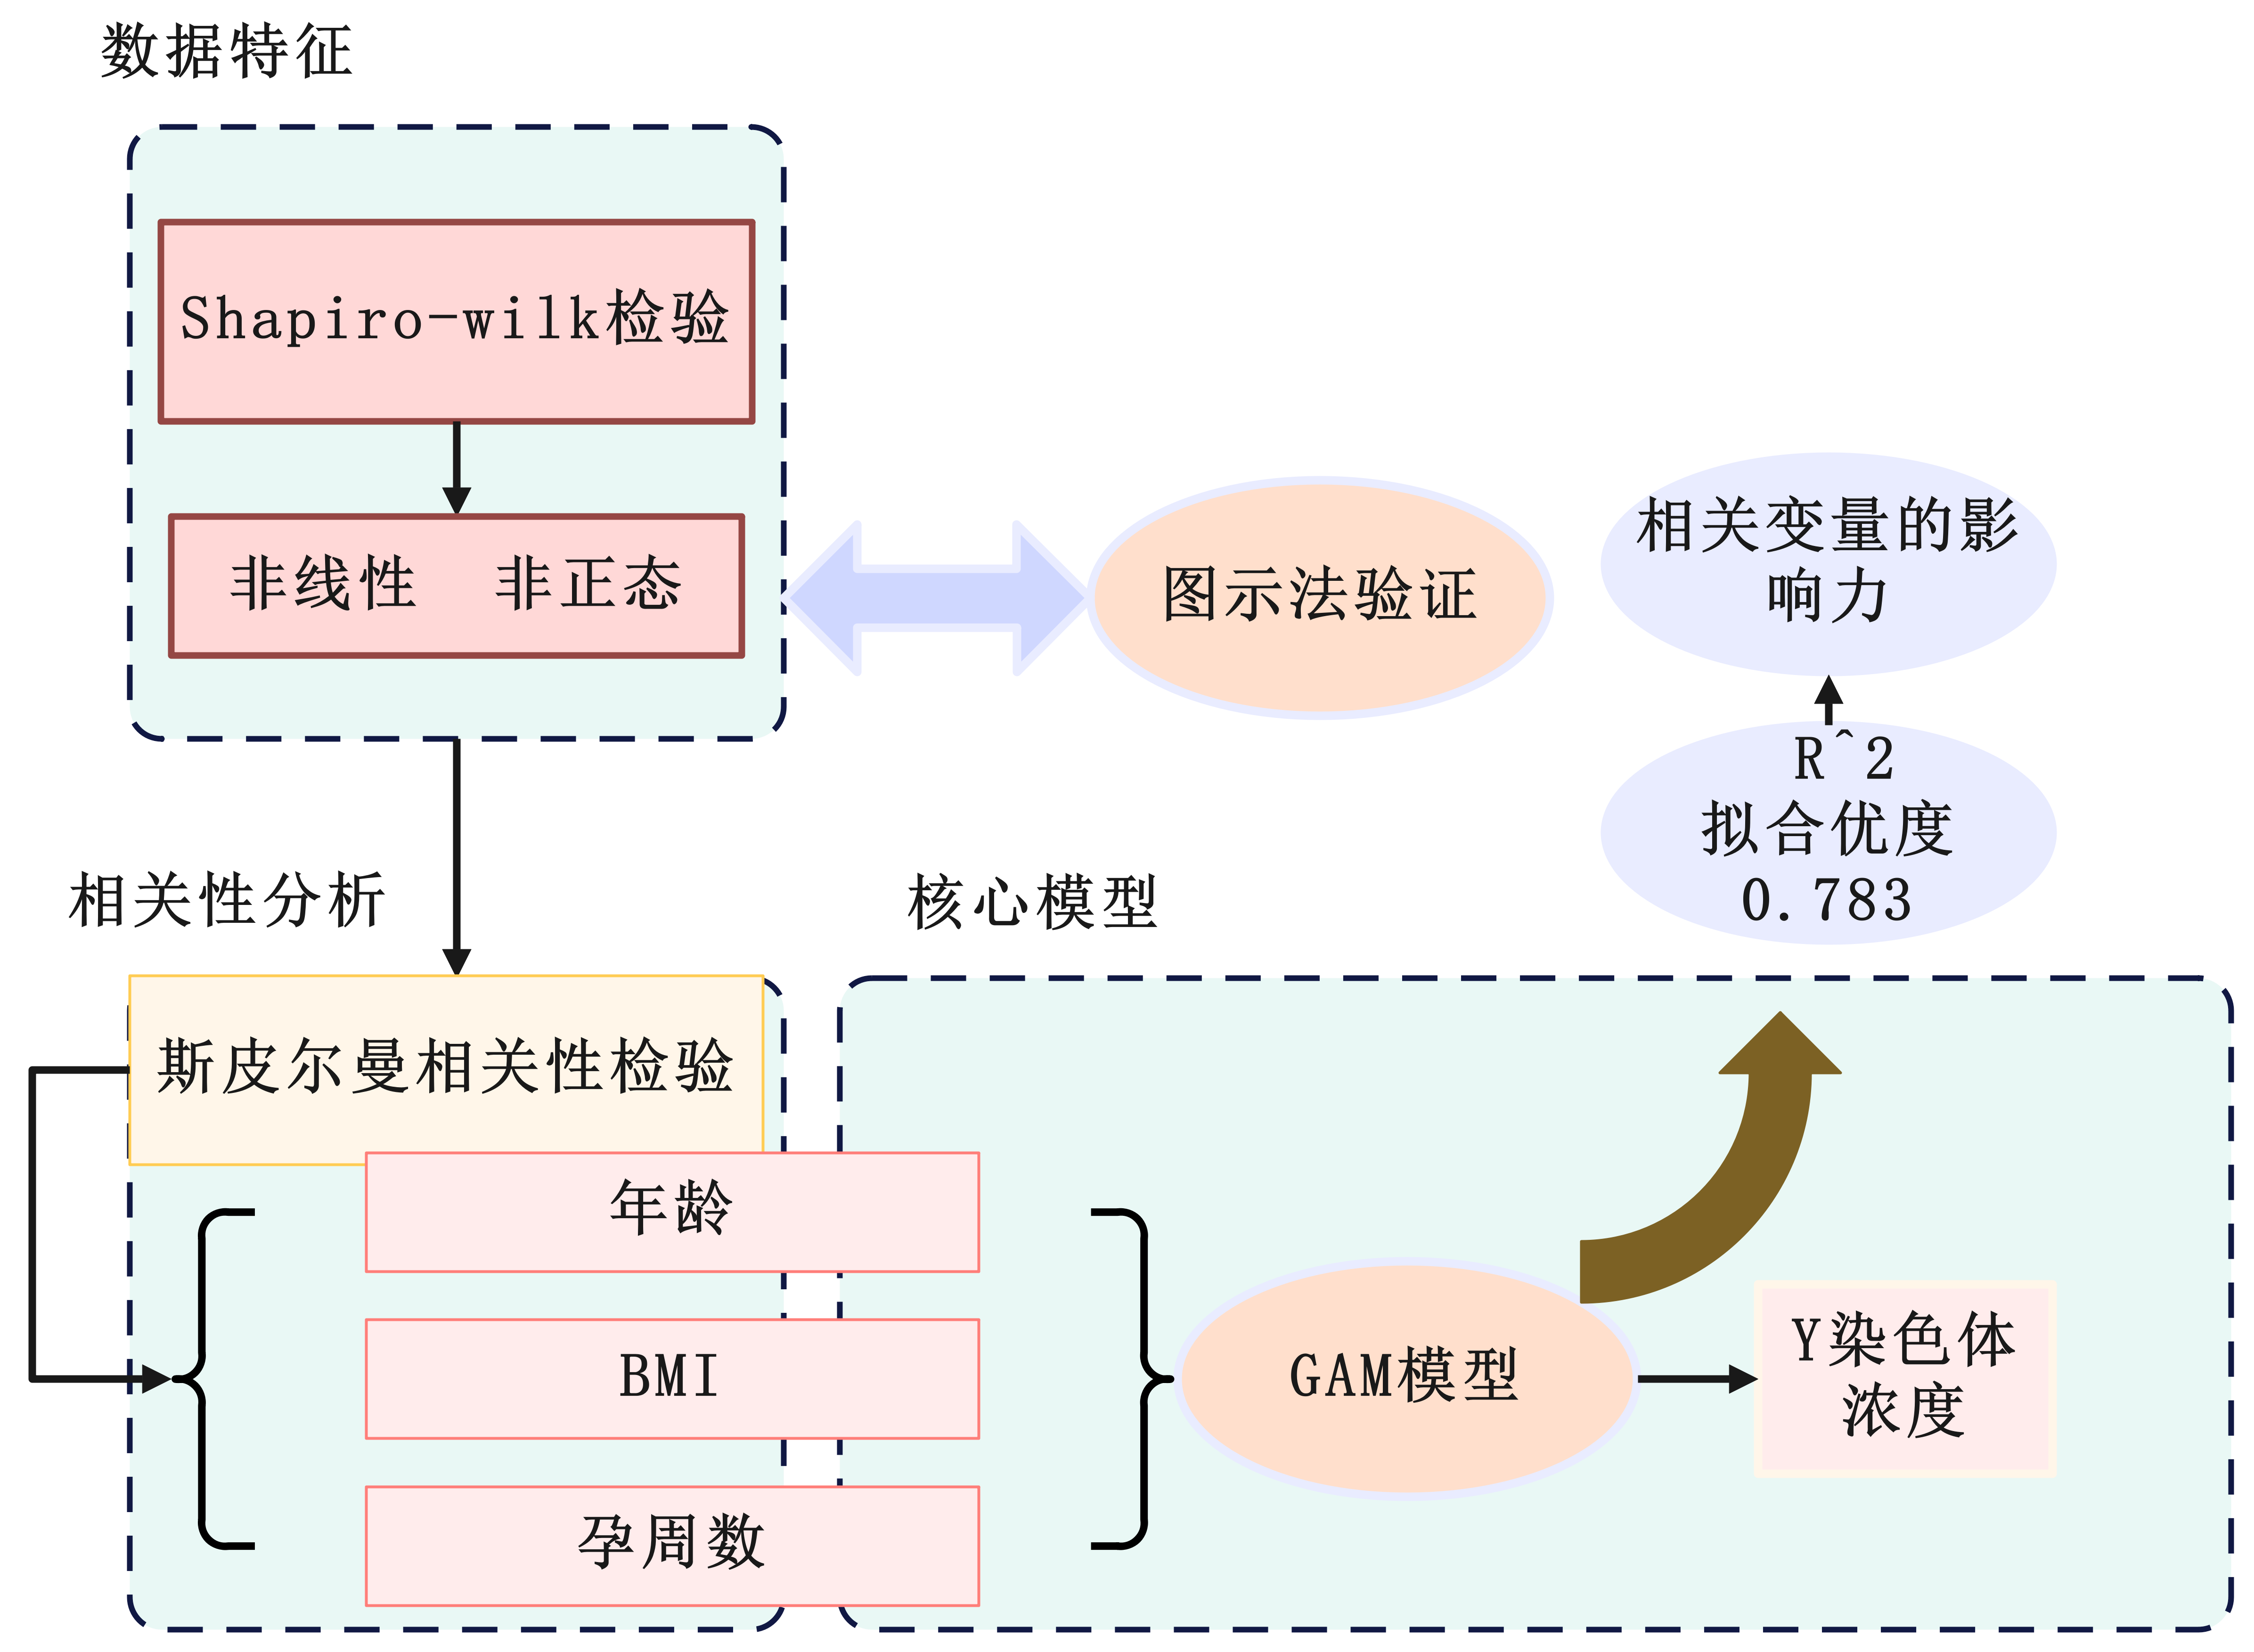
\includegraphics[width=0.7\textwidth]{Q1lc.png} % 图片路径和大小
		\caption{问题一流程图}
	\end{figure}
	
	\textbf{对于问题一},本文通过\textbf{Shapiro-Wilk检验}与\textbf{分层分析}的方法发现男胎$Y$染色体浓度分布是\textbf{非正态、非线性}的,不能使用依赖于正态分布的参数检验方法处理$Y$染色体浓度与孕妇的检测孕周和其 BMI 等指标的相关性,对此我们使用对非线性、无明显分布特征的关系能够有效衡量的\textbf{斯皮尔曼秩相关系数},得出了显著影响男胎$Y$染色体浓度的因素有孕妇年龄、孕妇BMI和检测孕周。对于非线性、非正态的特点,我们采用\textbf{广义加性模型(Generalized Additive Model, GAM)}对孕妇$Y$染色体浓度与其相关因素建立相应的关系模型,并且通过\textbf{McFadden伪$R^2$}说明该模型具有较好的拟合优度。

	\begin{figure}[htbp]
		\centering
		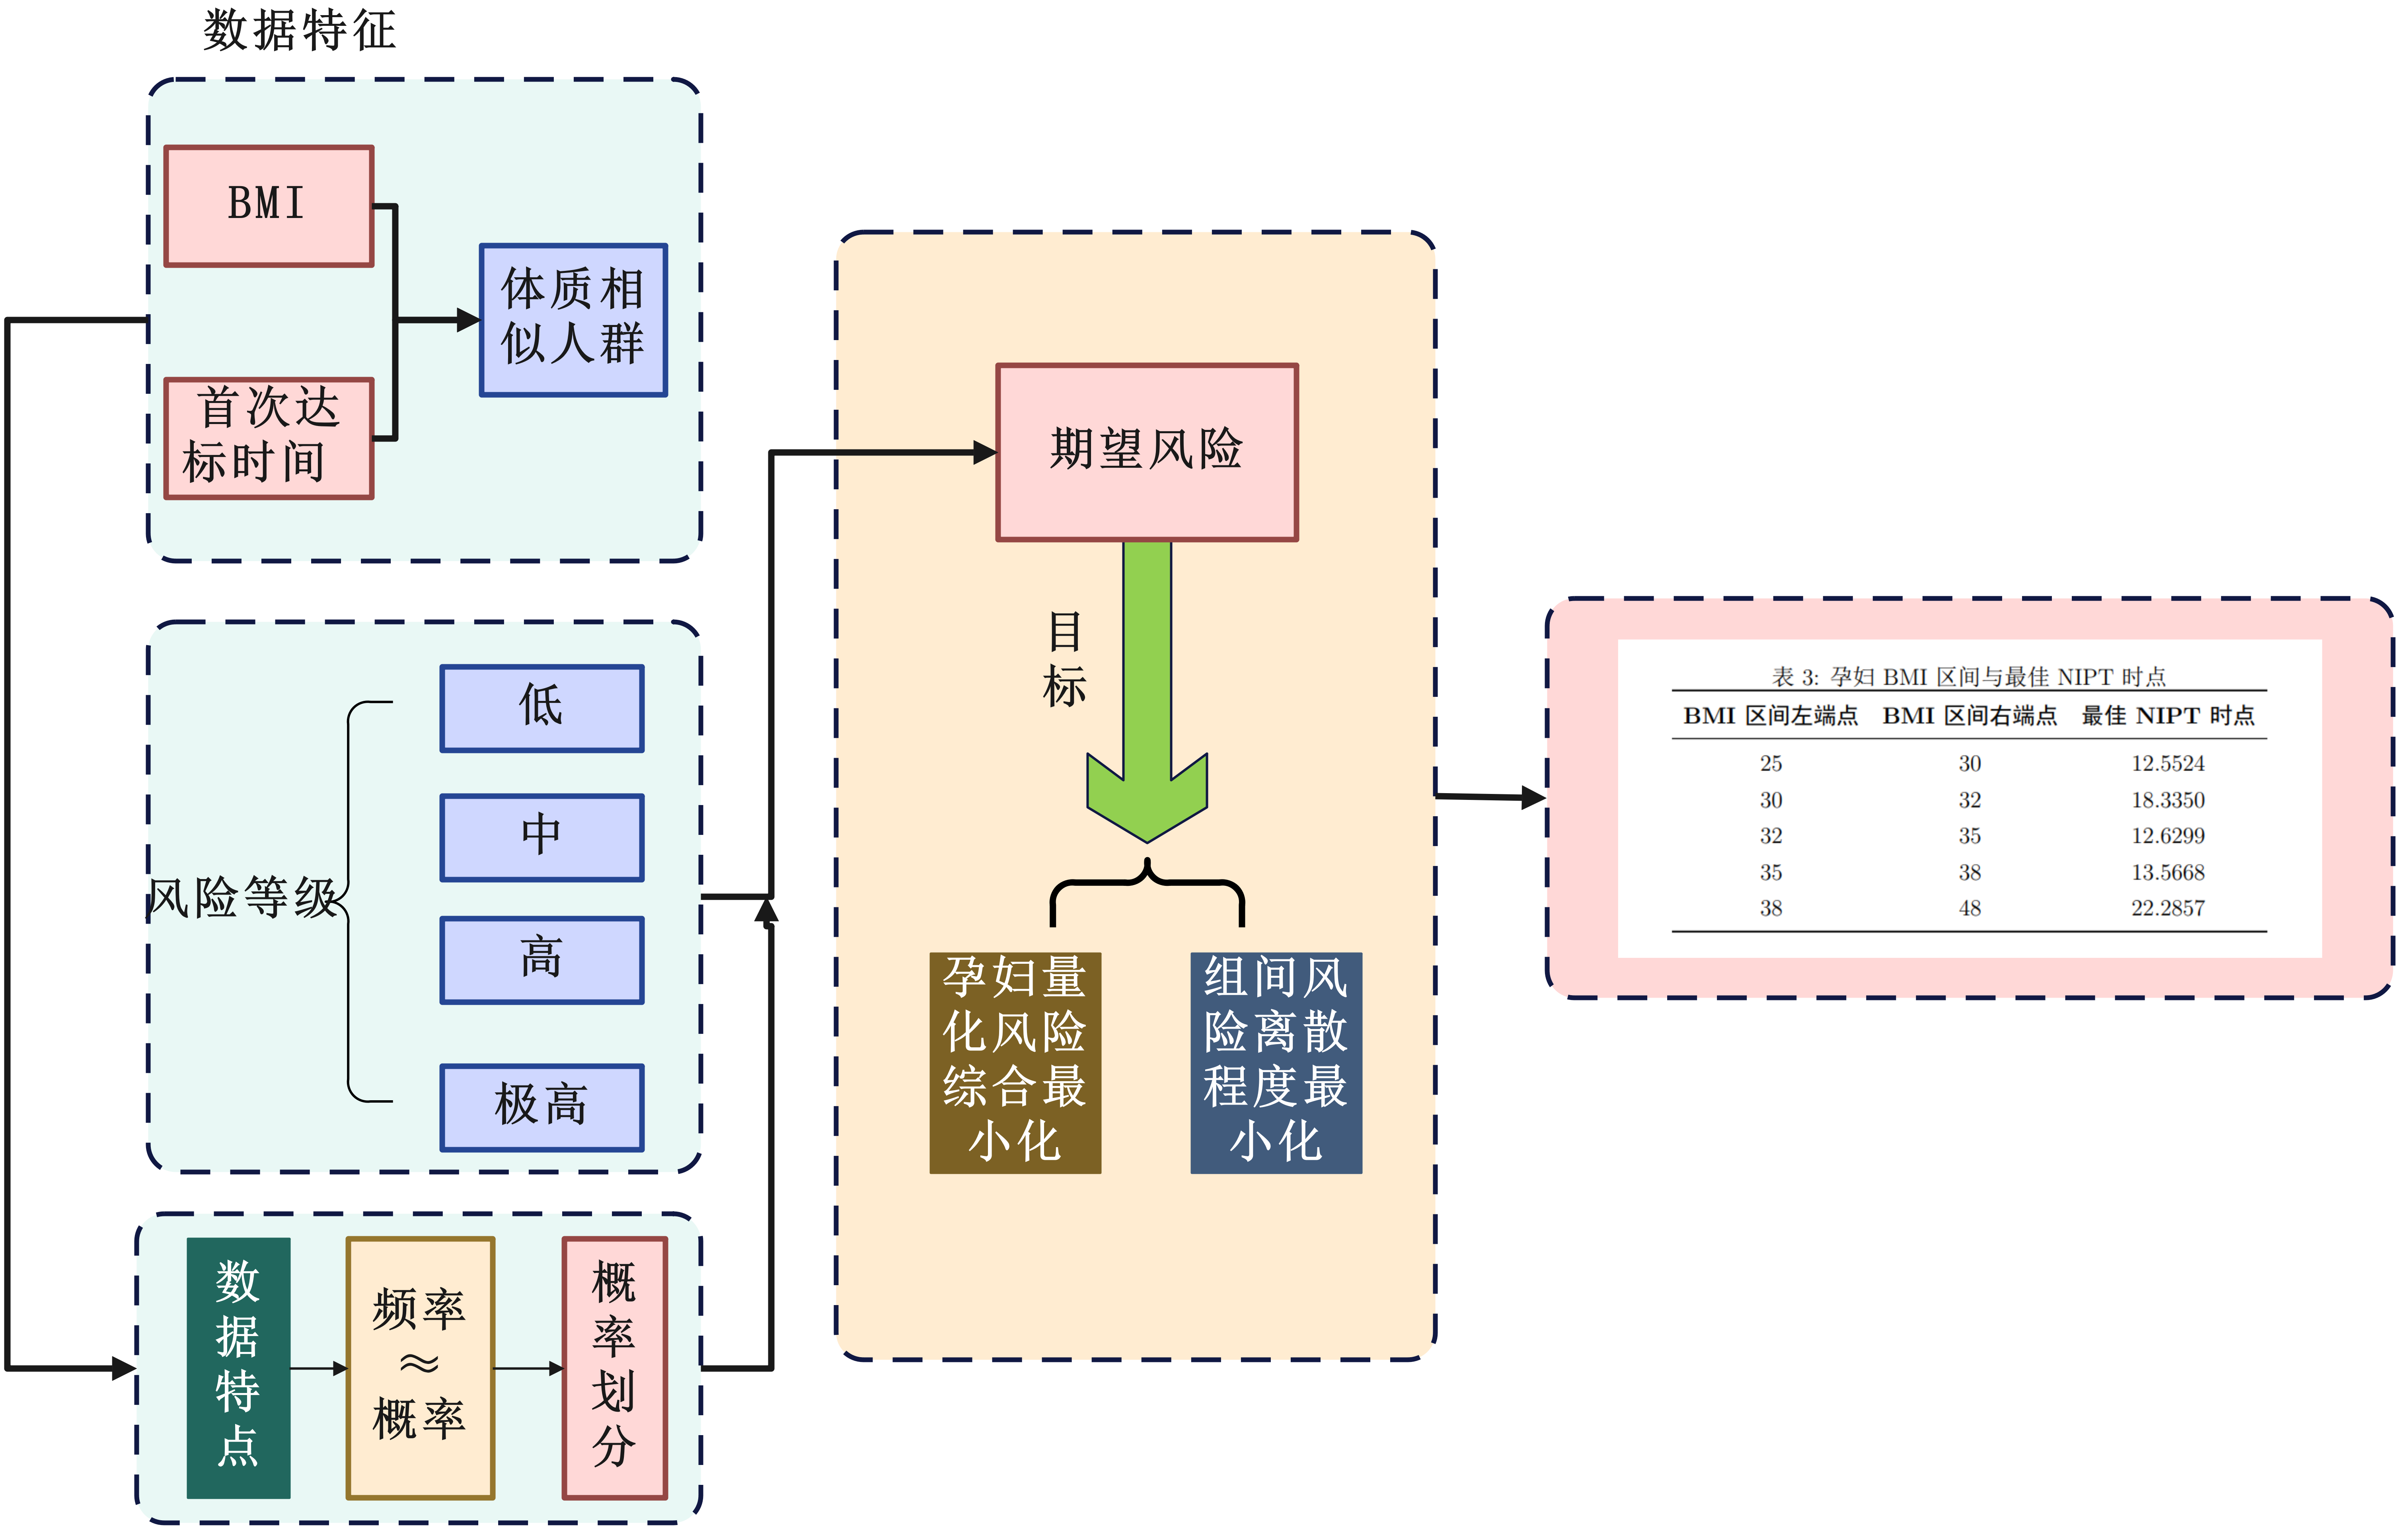
\includegraphics[width=0.98\textwidth]{Q2lc.png} % 图片路径和大小
		\caption{问题二流程图}
	\end{figure}
	
	\textbf{对于问题二},本文采用\textbf{分组--风险概率建模--风险期望评估}的思路,孕妇最佳NIPT时点与个体的生理特征有关,并且孕妇的BMI及其$Y$染色体浓度首次达标的时点能够有效刻画她们的体质特征,因此采用以孕妇BMI以及其$Y$染色体浓度首次达标的时点所构成的(BMI,T)二元数据组为聚类特征,使用K-means聚类方法进行聚簇分组。为了客观地评价风险程度,本文对风险程度进行了量化赋值,并结合了数据量较大的特点,构建了\textbf{风险概率模型},二者结合刻画分组总体的风险总和以及风险离散程度,从而衡量分组的质量。后续引入高斯白噪声来模拟检测误差,多次求解后的结果说明模型具有较好的的鲁棒性。
	
	\begin{figure}[H]
		\centering
		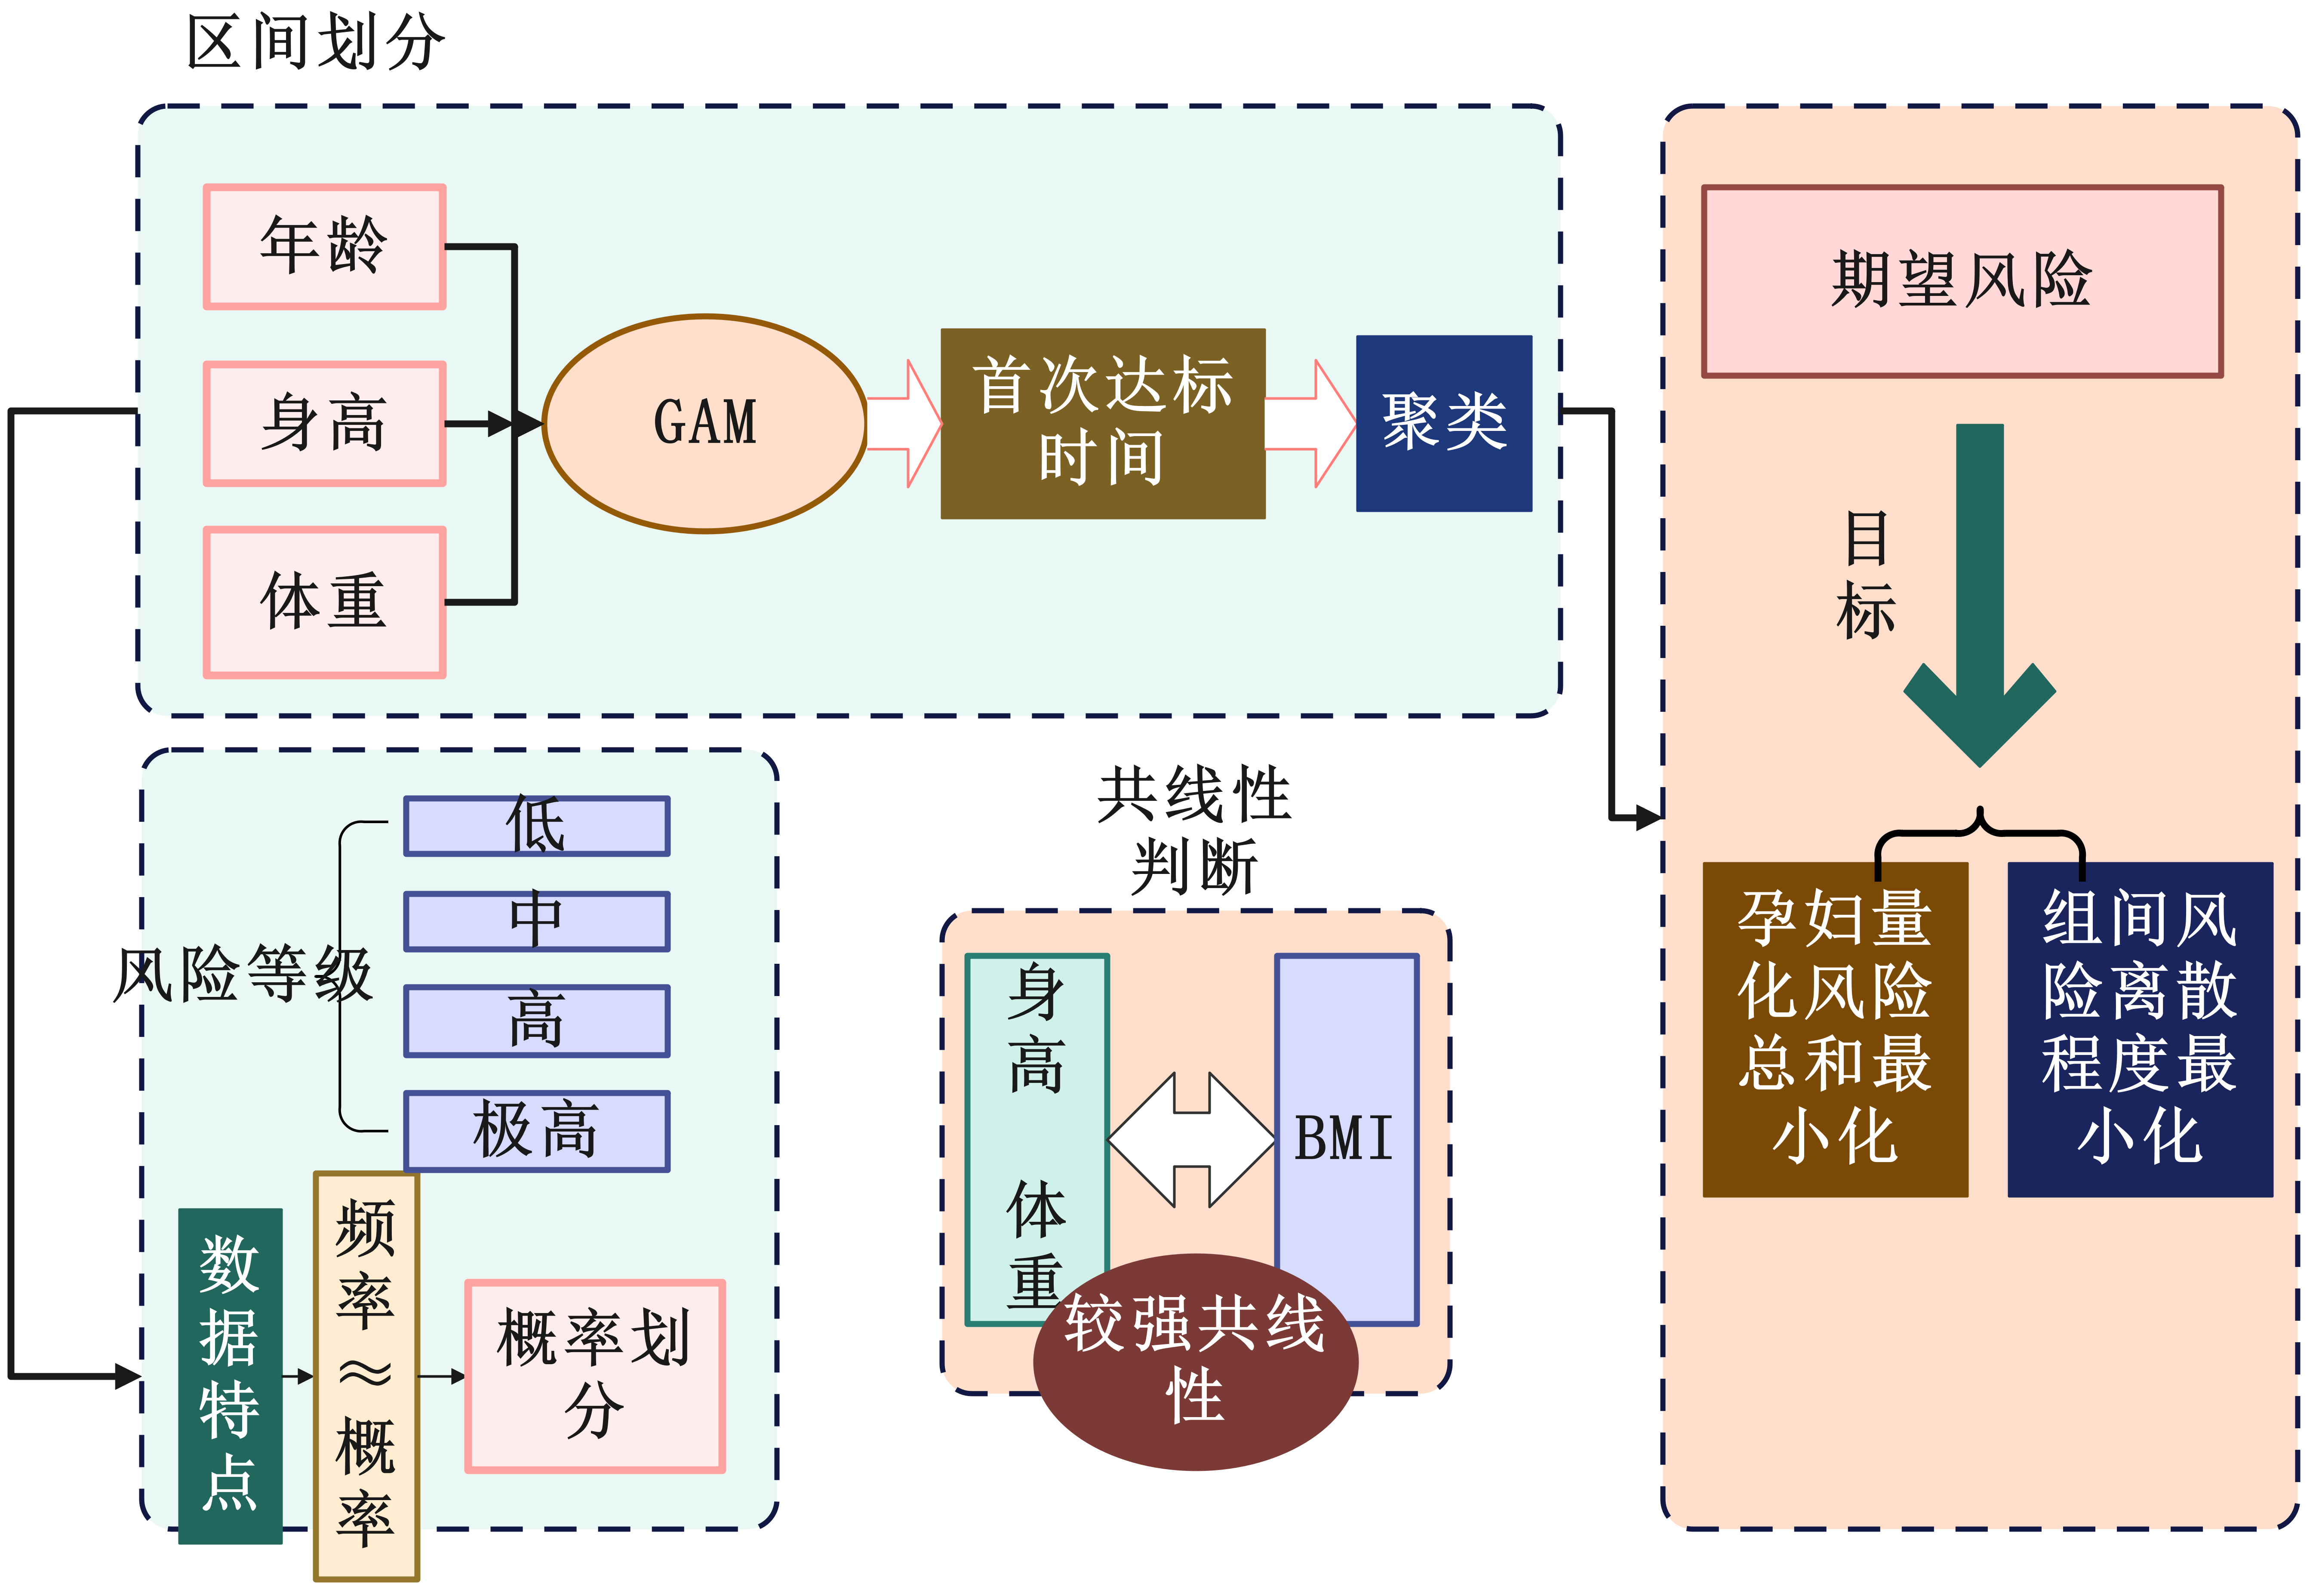
\includegraphics[width=0.7\textwidth]{Q3lc.png} % 图片路径和大小
		\caption{问题三流程图}
	\end{figure}

	\textbf{对于问题三},本文采用\textbf{共线性检测--预测模型--区间划分--风险期望评估的思路},进一步引入了孕妇年龄、身高、体重等影响因素。首先通过共线性检测,验证了孕妇BMI与身高体重具有\textbf{显著的共线性},于是使用BMI代替身高体重对分组的影响,以简化模型结构,避免多重共线性的影响。
	
	BMI区间划分的最终目的是刻画最佳NIPT时点,使得孕妇可能的潜在风险最低,即进行NIPT检测越早越好,本文首先通过相关性分析选定特征变量,进而构建\textbf{广义可加模型(GAM)},以孕妇年龄,BMI,以及$Y$染色体浓度为输入拟合检测孕周,再将$Y$染色体浓度为\textbf{4\%}代入数据,得到每个孕妇$Y$染色体浓度首次达标时间点,再结合BMI和年龄进行\textbf{K-means聚类},针对不同分组,使用与问题二一致的量化风险评价指标进行风险评估。最后再引入\textbf{高斯白噪声}进行检测误差的扰动,结果表明,相较于问题二的模型,本题提出的多变量聚类模型在风险控制方面表现更优,且具有更高的稳定性。
		
		\begin{figure}[H]
		\centering
		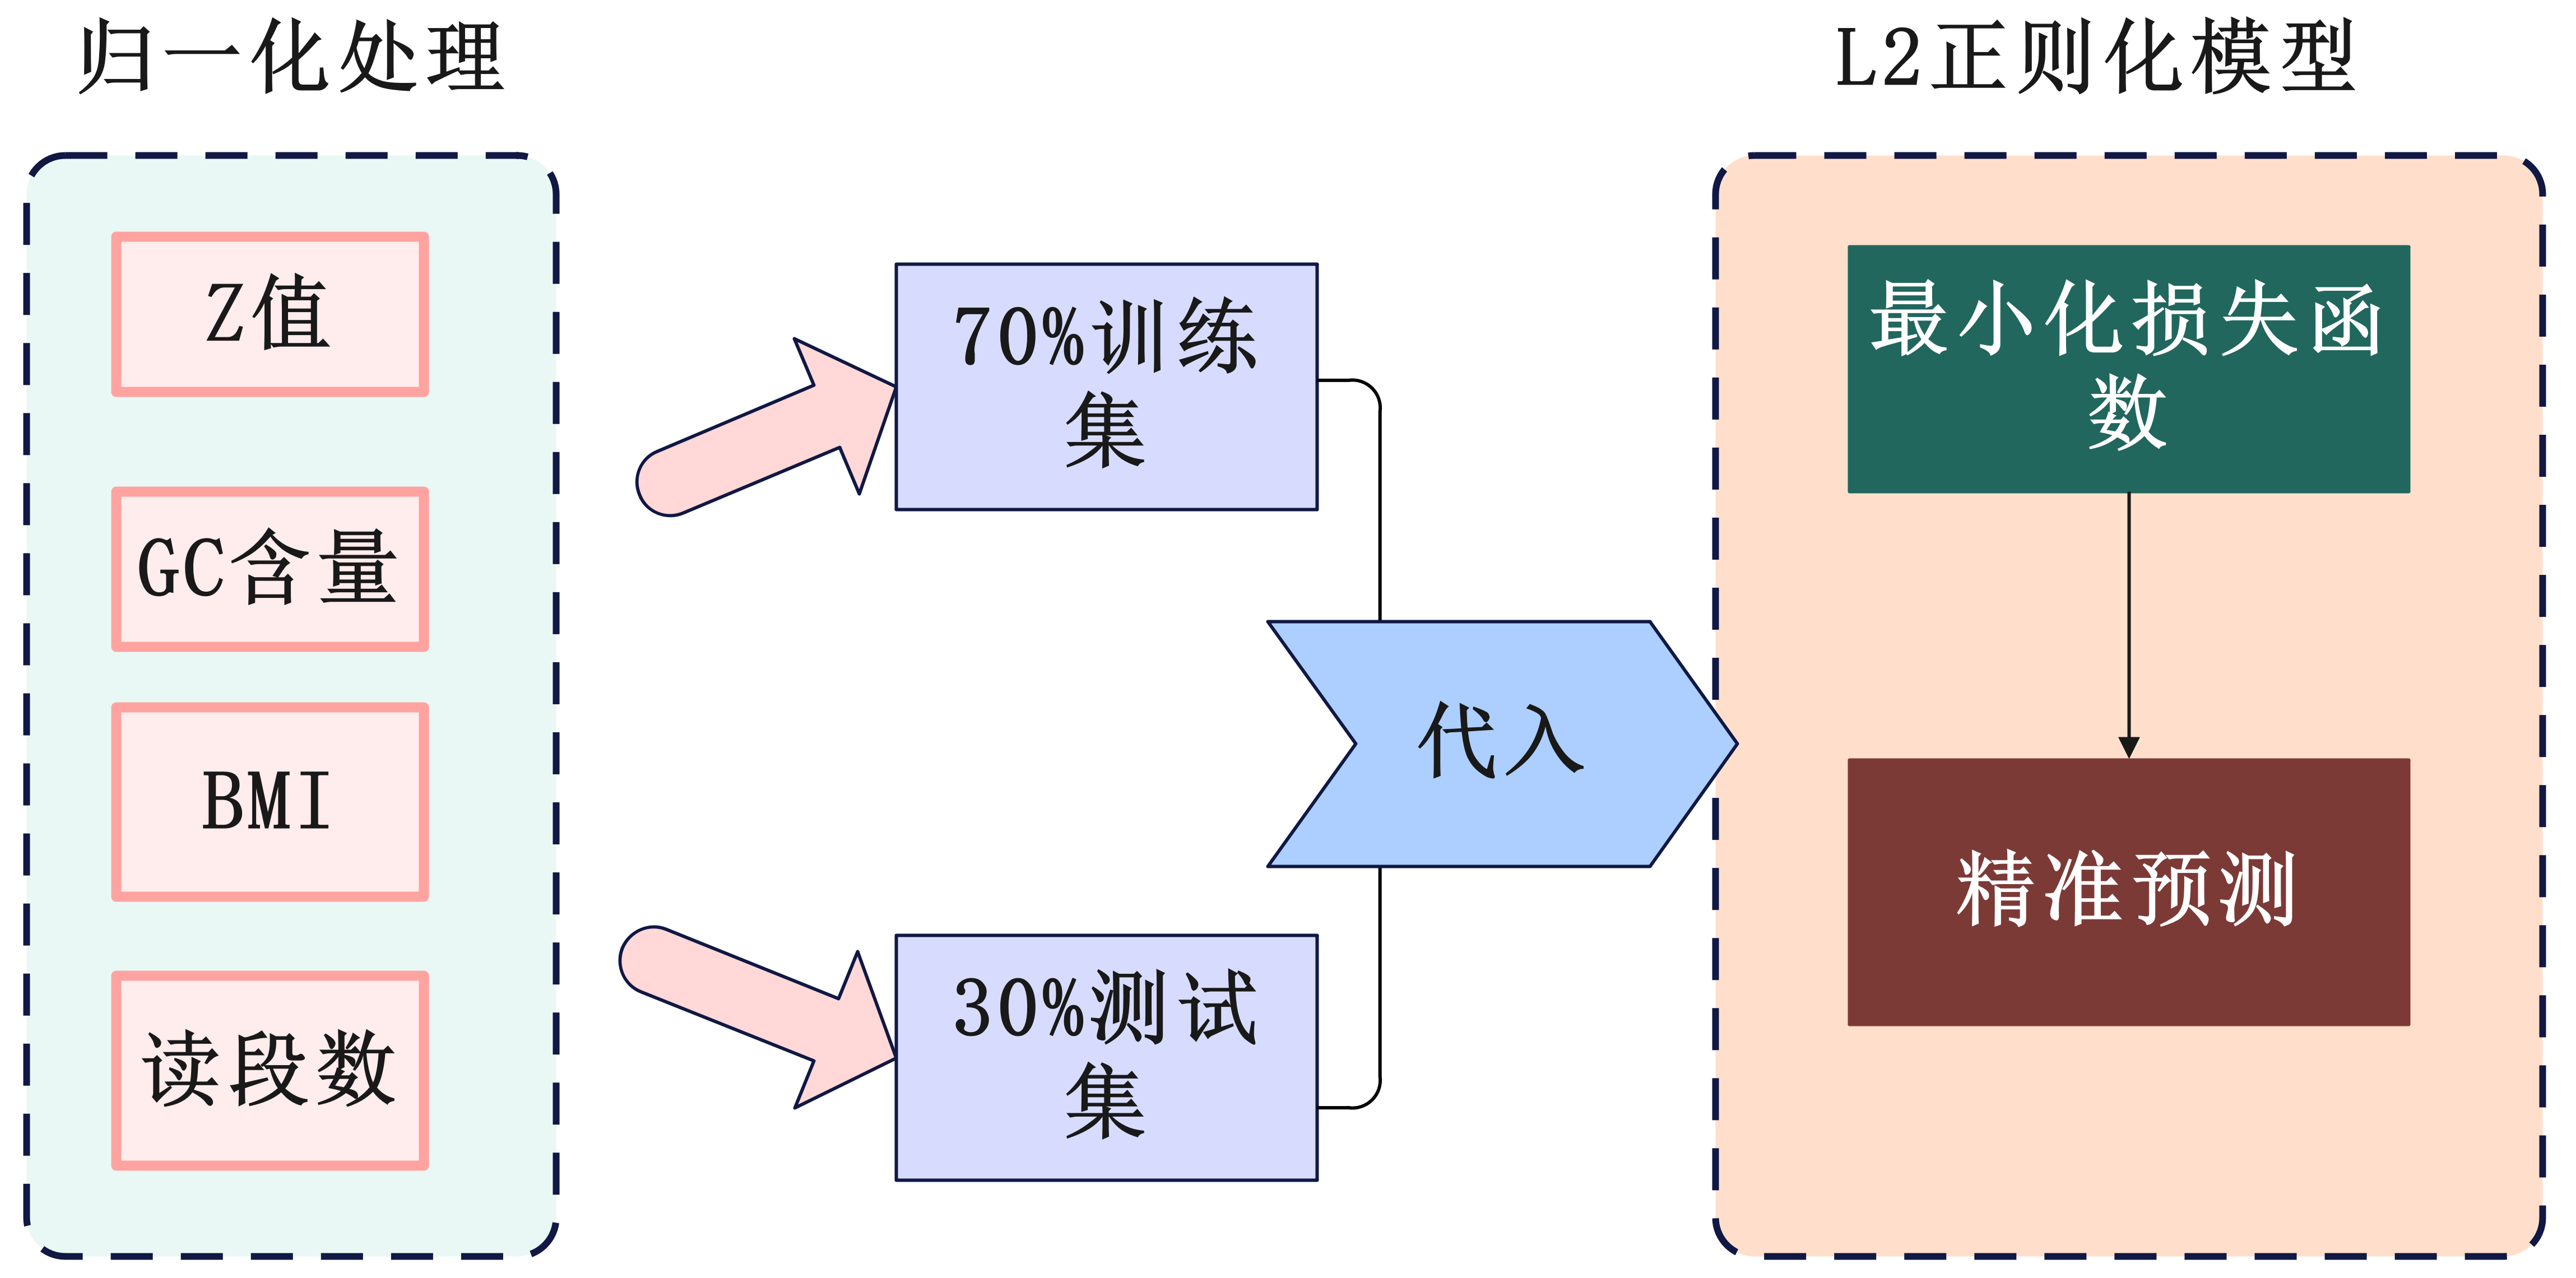
\includegraphics[width=0.65\textwidth]{Q4lc.png} % 图片路径和大小
		\caption{问题四流程图}
	\end{figure}
	
	\textbf{对于问题四},主要问题是如何判断NIPT中的染色体异常数据,特别是在数据严重不平衡的情况下进行准确分类。由于异常样本仅占总样本的\textbf{$\frac{1}{10}$},传统分类算法在此情况下容易偏向于预测正常类,从而影响模型性能。因此,本文选择了\textbf{带L2正则化的逻辑回归模型},L2正则化有助于减轻过拟合并提高模型的泛化能力,特别是对少数类样本的预测能力。为了确保模型能够公平处理不同尺度的特征,本文对与染色体异常相关的多个特征(如Z值、GC含量、BMI、读段数等)进行了\textbf{归一化处理}。经过归一化处理后,模型能够更好地识别这些特征与染色体异常之间的关系。评估模型时,本文采用了\textbf{准确率(Accuracy)}指标,结果显示模型具有优异的准确性。
		
	
	\section{模型假设}
	1.假设样本量具有代表性,同时数据真实可靠,能够反应真实NIPT检测的规律。
	
	2.假设假定数据中出现的缺失值在建模时可直接依据其生物学意义进行处理,且不会对模型主体结构产生系统性偏差。
	
	3.假设孕妇的潜在风险与时间相关并能够被量化。
	
	\section{符号说明}
	
	\begin{table}[H]
		\centering
		\setlength{\tabcolsep}{12pt} % 调整列间距
		\begin{tabular}{@{}ll@{}}
			\toprule
			符号 & 说明 \\ \midrule
			$Y$ & 孕妇$Y$染色体浓度 \\
			$BMI$ & 孕妇BMI \\
			$Age$ & 孕妇年龄 \\
			$T$ & 孕妇$Y$染色体浓度首次达到4\%的检测孕周 \\
			$t$ & 孕妇的检测孕周 \\
			$\rho_{XY}$ & 斯皮尔曼相关系数\\
			$	R^2_{\text{McFadden}}$ & \text{McFadden}伪$R^2$\\
			$p_i$ & 各BMI分组种的第$i$种风险程度概率 \\
			$C(y,t)$ & 风险程度的定量化函数\\
			$K$ & 依据BMI分组的总组数 \\ 
			$\mathrm{Cov}(\varepsilon_t,\varepsilon_s)$ & 协方差 \\
			$\mu$ & 均值 \\ 
			$\sigma^2$ & 方差 \\
			$Accuracy$ & 带L2正则化的逻辑回归模型的准确性\\
			\bottomrule
		\end{tabular}
	\end{table}
	
	\newpage
	
	\section{问题一求解}
	
	\subsection{数据预处理}
	
	
	观察数据可知,附件数据表格中的检测孕周列(J列)的数据不可直接使用,所以我们将其统一转换为以周为单位,并保留四位小数的数值型数据。通过查阅相关文献\cite{wang2013},\textbf{孕妇年龄}、\textbf{孕妇BMI}以及\textbf{检测孕周}与男胎$Y$染色体浓度具有显著相关性。
	
	\subsection{相关性分析}
	为了验证上述假设,本文采用图示法与相关性检验对附件数据进行了相关性分析。
	
	\subsubsection{图示法}
	考虑到多个影响因素与孕周数并列存在,无法相对独立的观察单一因素对待测变量的影响。为控制这些混杂因素,本文采用了\textbf{分层分析}的方法。为了研究孕周数对$Y$染色体浓度的影响,取样本量最集中的年龄28岁进行分析,接着将BMI进行\textbf{四分位分组},在每个亚组中,$Y$染色体浓度与孕周数的变化独立显现,显著降低了其他因素的混杂影响。下图为孕周数与$Y$染色体浓度的散点图:
	\begin{figure}[htbp]
		\centering
		% 第一行
		\subfigure[检测孕周11-14]{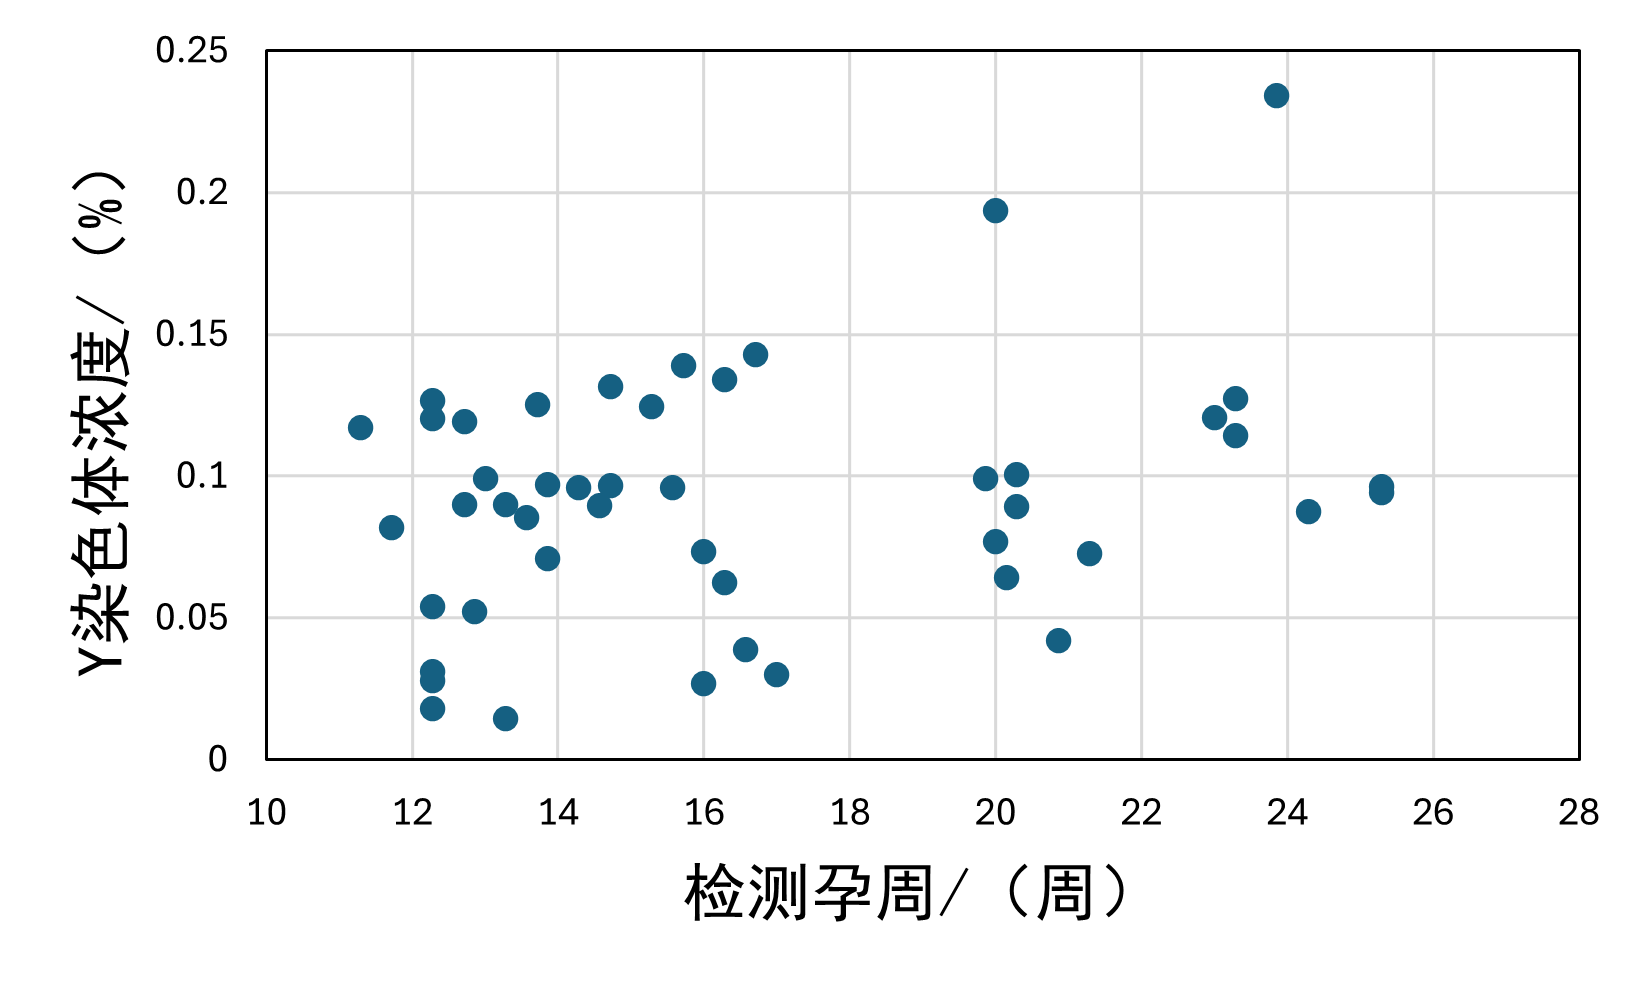
\includegraphics[width=0.4\textwidth]{ga11-14.png}}
		\subfigure[检测孕周14-17]{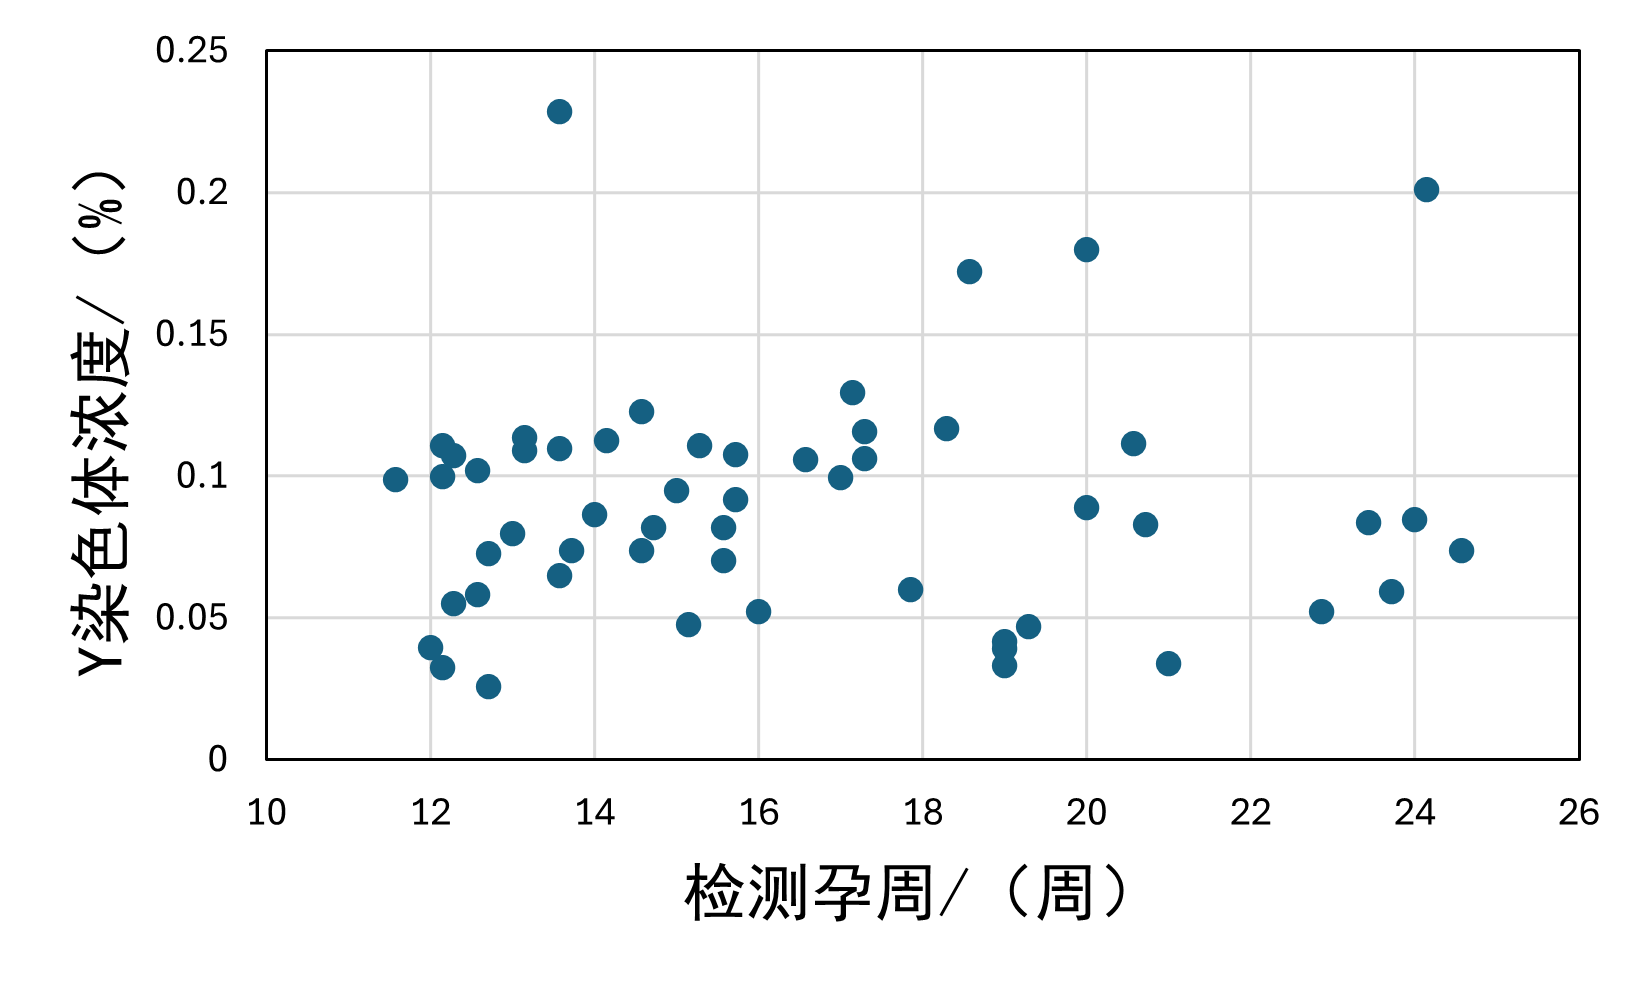
\includegraphics[width=0.4\textwidth]{ga14-17.png}} \\[1ex]
		% 第二行
		\subfigure[检测孕周17-20]{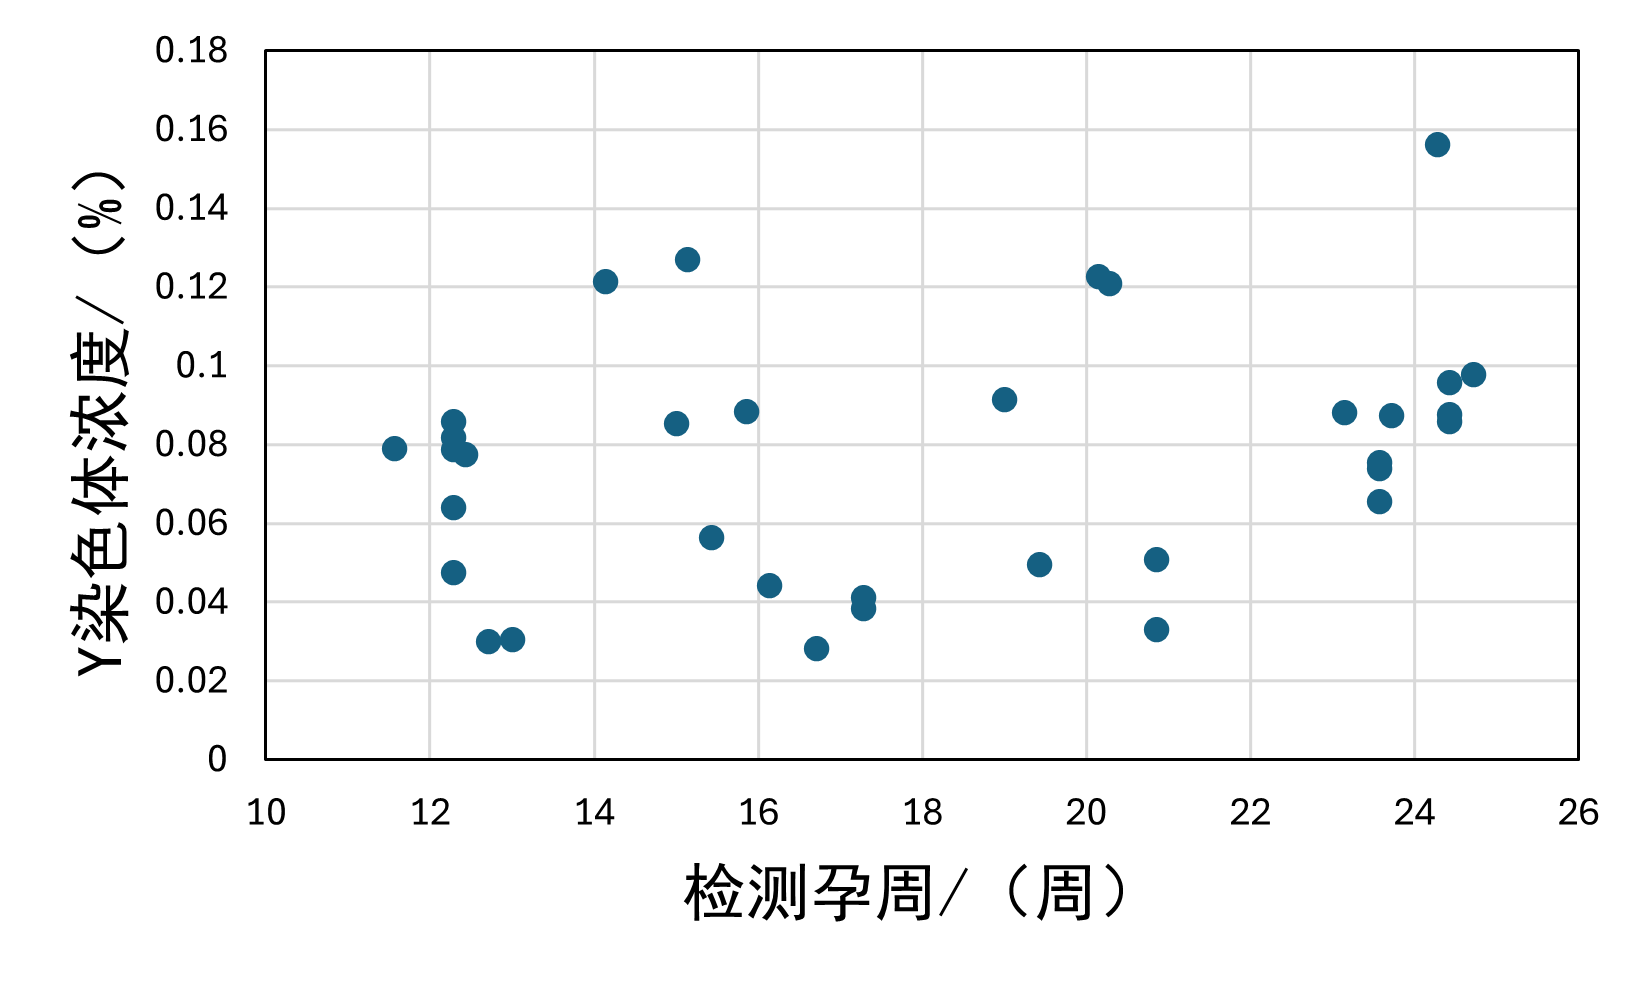
\includegraphics[width=0.4\textwidth]{ga17-20.png}}
		\subfigure[检测孕周20-23]{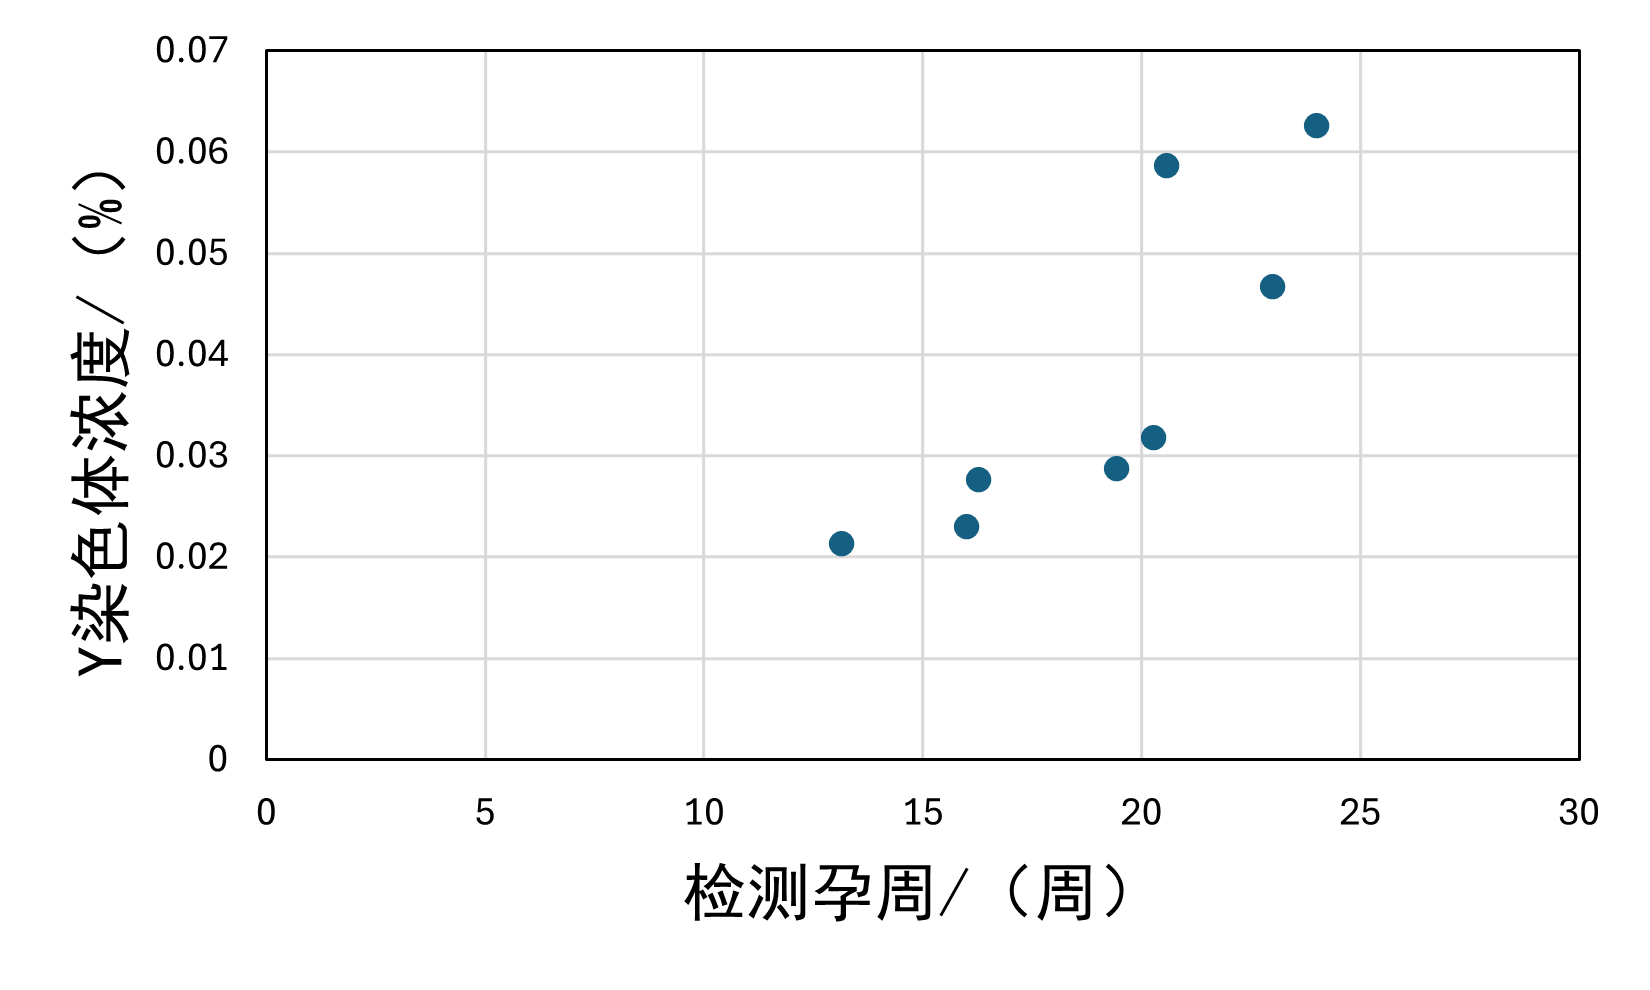
\includegraphics[width=0.4\textwidth]{ga20-23.png}}
		\caption{$Y$染色体浓度与检测孕周的散点图}
	\end{figure}
	
	以上散点图直观地体现了$Y$染色体浓度随着孕周数的增加具有一定的\textbf{上升趋势},同时具有较强的\textbf{非线性}关系。

	
		同样的,在研究BMI对$Y$染色体浓度的影响时,为了修正孕周数对BMI的混杂影响,我们将检测孕周以\textbf{3}为步长分为四组,在各个亚组中研究$Y$染色体浓度随BMI的变化关系,得到以下散点图:
		\begin{figure}[htbp]
			\centering
			% 第一行
			\subfigure[孕妇BMI 27-30]{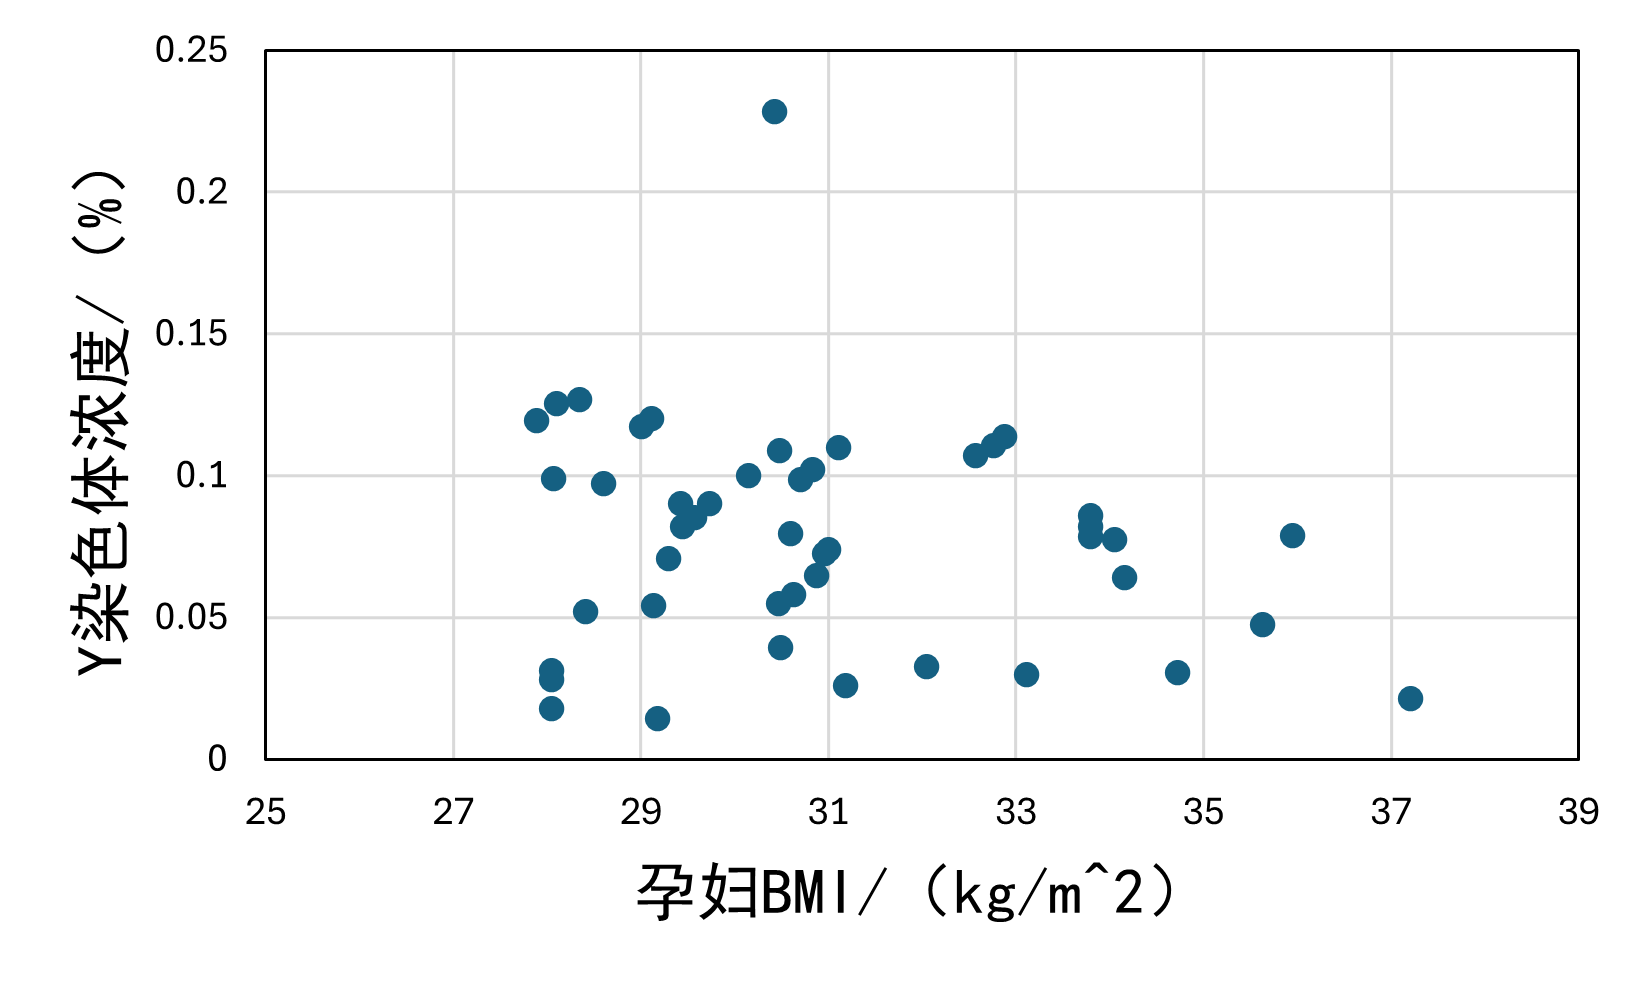
\includegraphics[width=0.4\textwidth]{BMI27-30.png}}
			\subfigure[孕妇BMI 30-33]{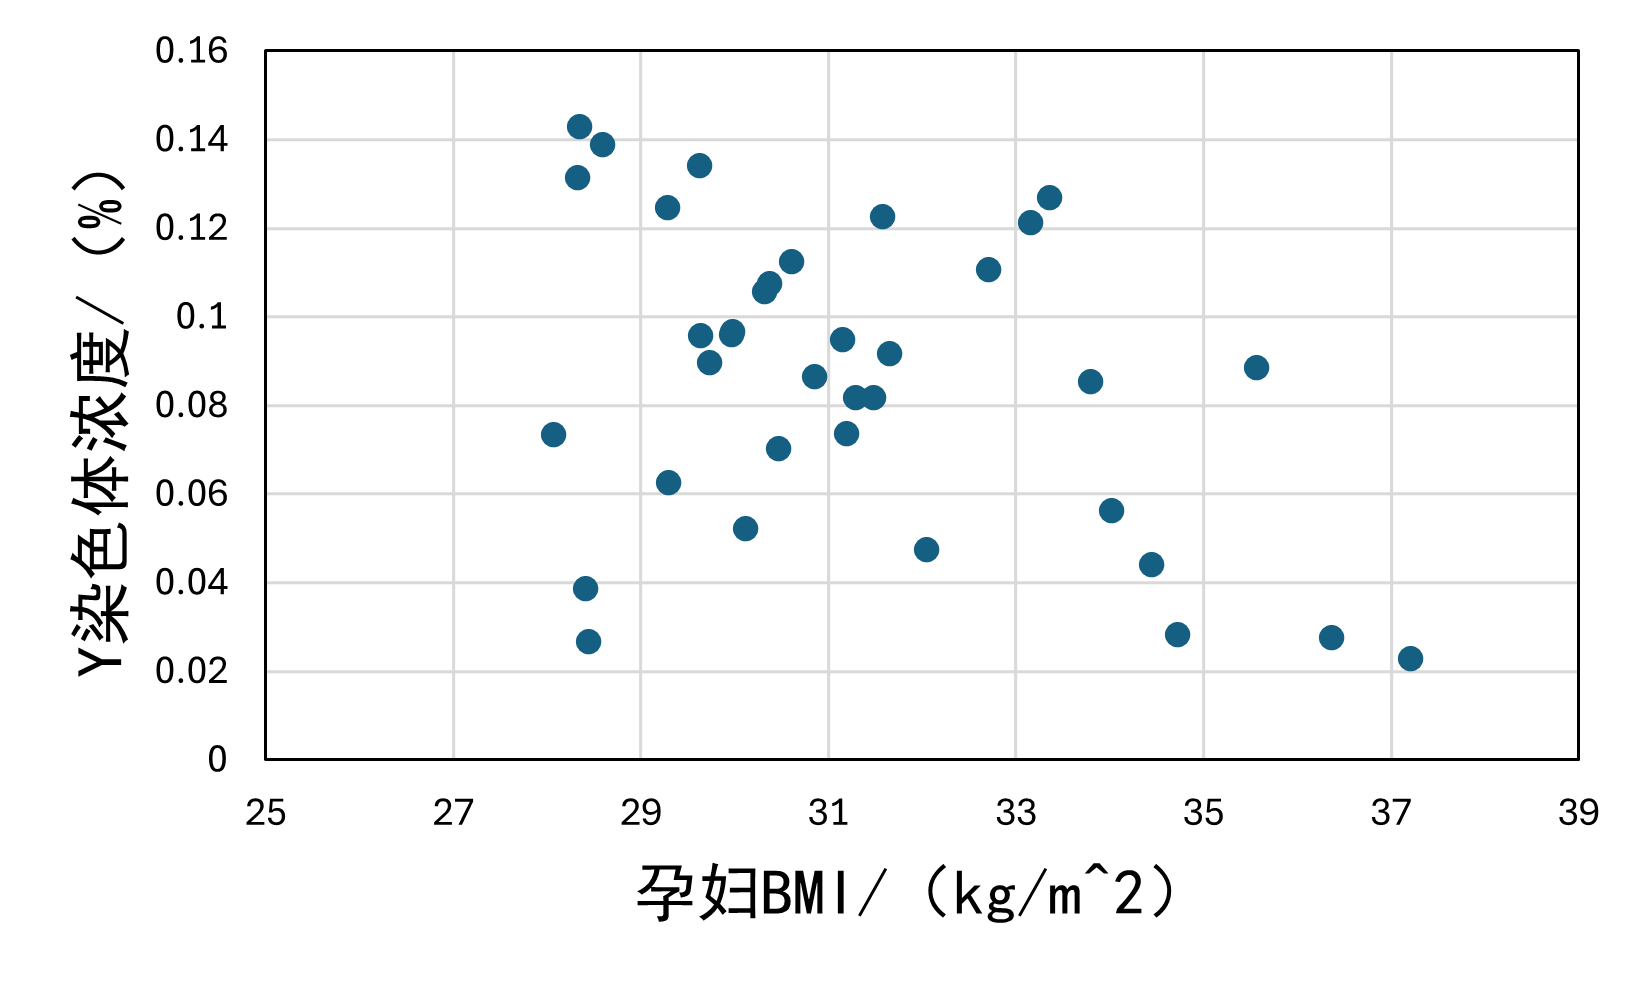
\includegraphics[width=0.4\textwidth]{BMI30-33.png}} \\[1ex]
			% 第二行
			\subfigure[孕妇BMI 33-36]{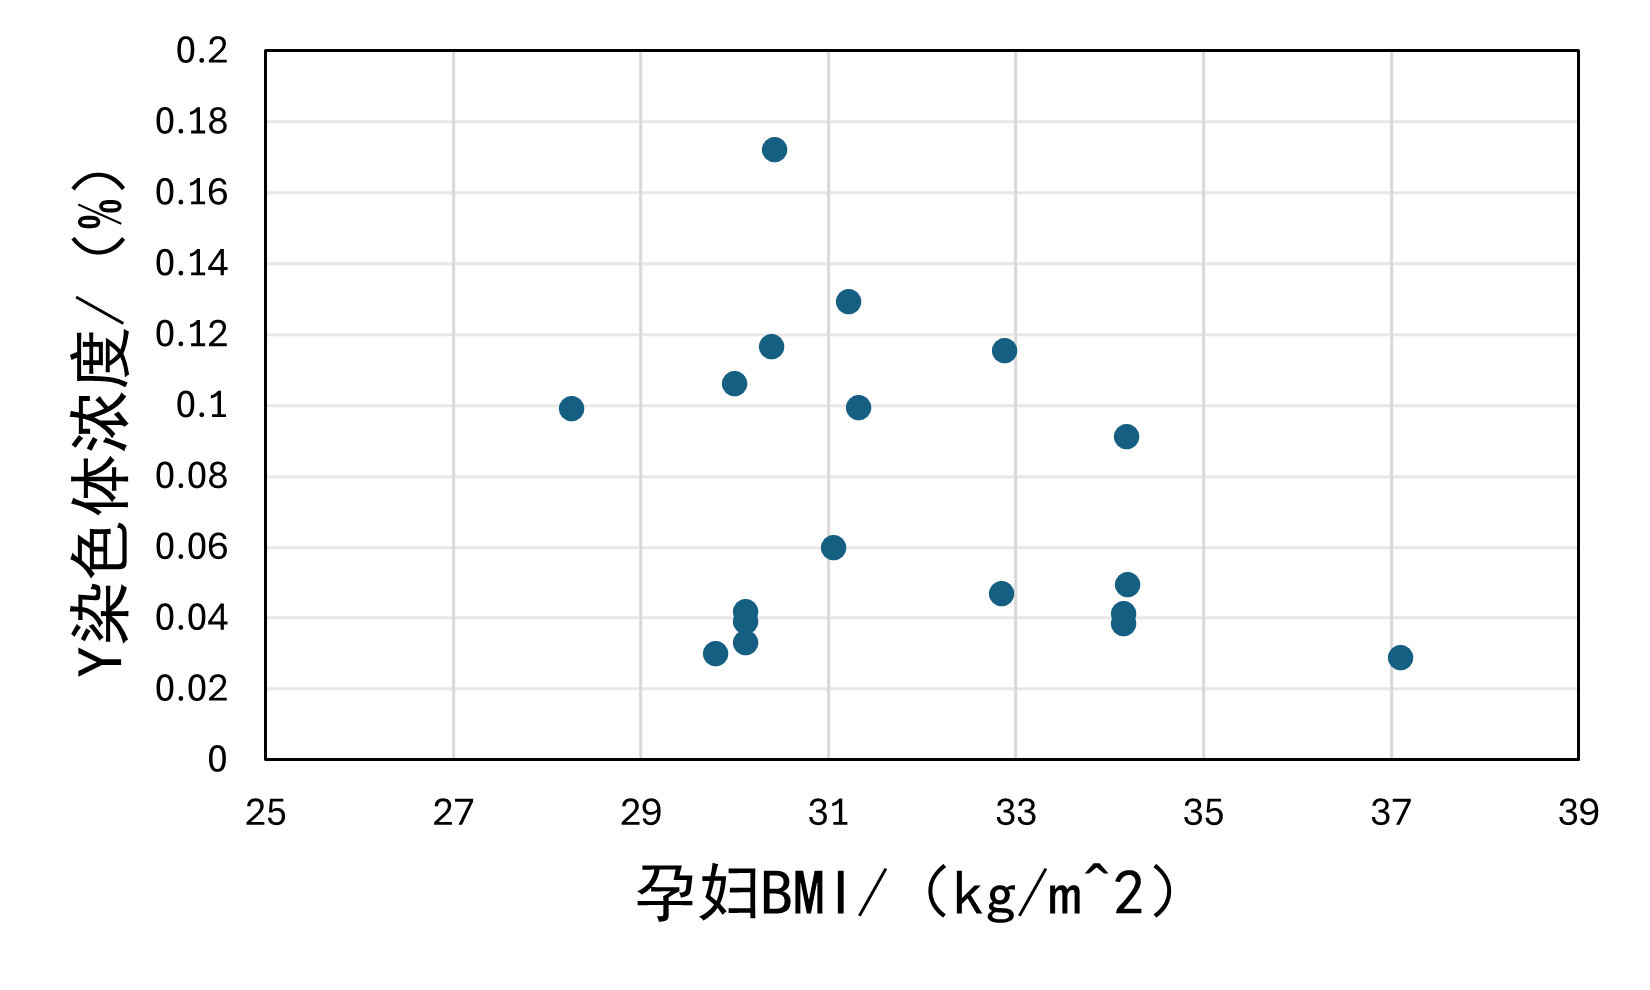
\includegraphics[width=0.4\textwidth]{BMI33-36.png}}
			\subfigure[孕妇BMI 36-39]{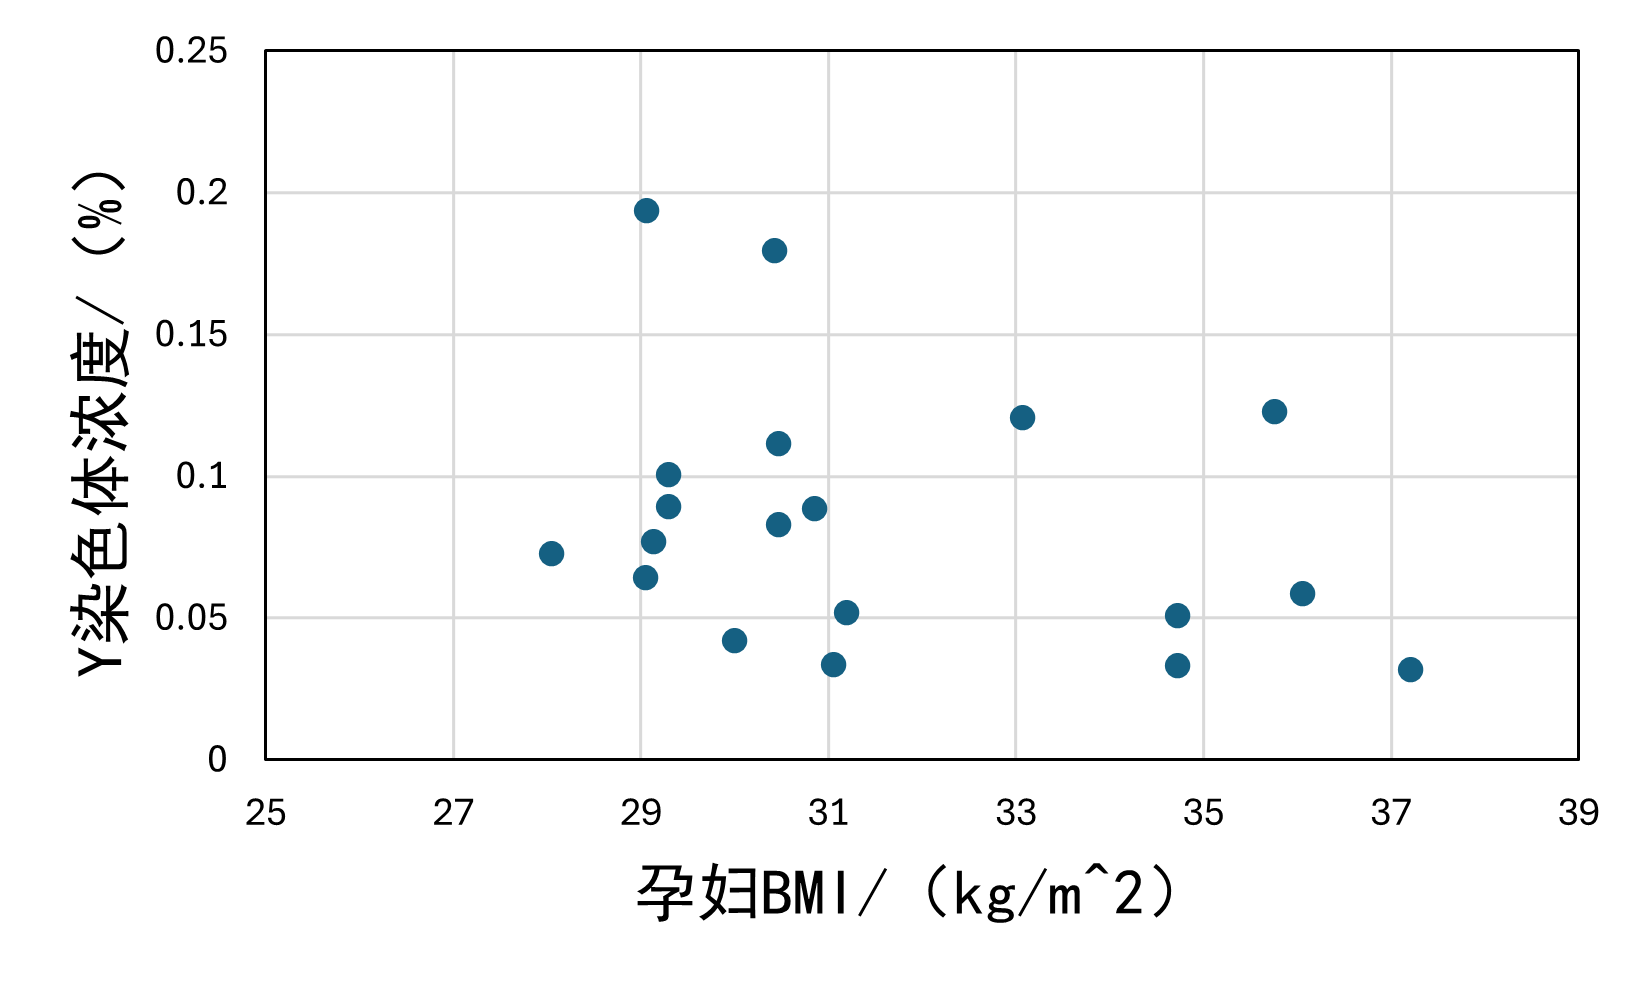
\includegraphics[width=0.4\textwidth]{BMI36-39.png}}
			\caption{$Y$染色体浓度与孕妇BMI的散点图}
		\end{figure}

	
	与孕周数结果相同的是,两者都具有较强的、\textbf{非线性关系};但在相同孕周数内,$Y$染色体浓度随着BMI的增加出现了\textbf{先增加后降低}的趋势。\cite{canick}虽未直接给出BMI对$Y$染色体浓度的影响,但提到了$Y$染色体浓度会随孕周数的增加呈现\textbf{上升的趋势},随孕妇体重的增加呈\textbf{下降趋势};我们发现,在BMI的定义中体重为平方项,因此在BMI增长前期出现上升趋势,后随体重增加会出现下降趋势,与本题所给数据相契合。
	
	而\textbf{对于孕妇年龄}因素,我们将每个年龄的孕妇作为一组,将所有该年龄的孕妇的$Y$染色体浓度取均值,得到以下散点图:
	\begin{figure}[H]
		\centering
		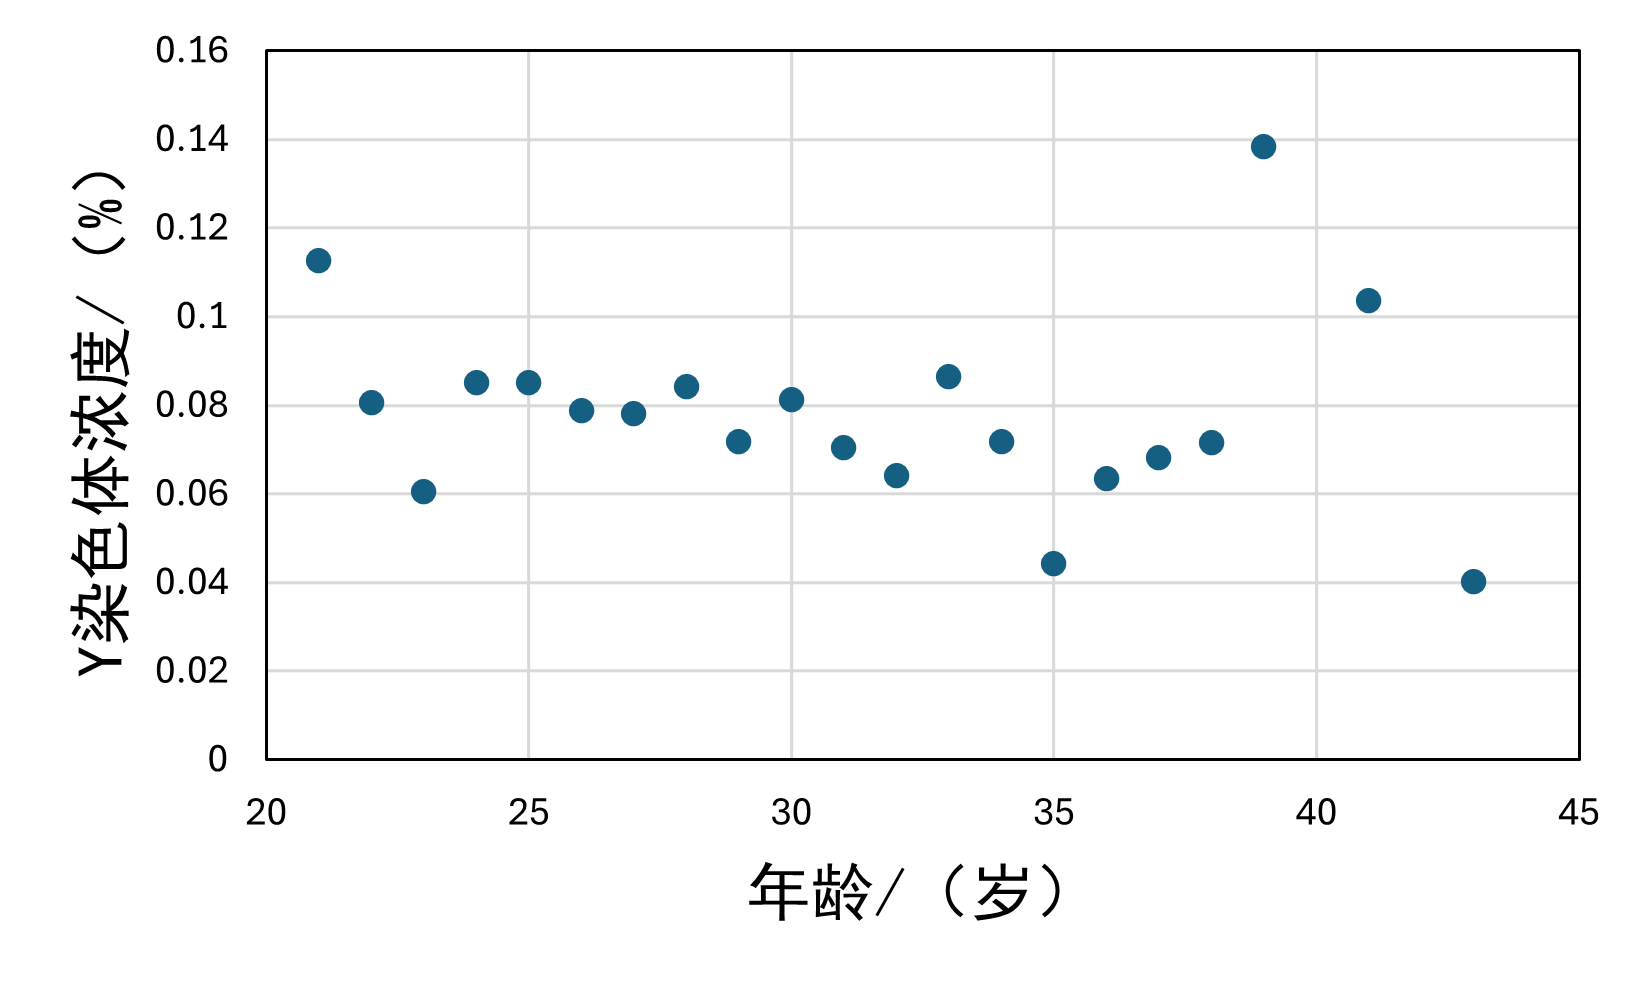
\includegraphics[width=0.4\textwidth]{age.png} % 图片路径和大小
		\caption{$Y$染色体浓度与孕妇年龄散点图}
		\label{fig:example}
	\end{figure}
	
	我们发现,在排除了部分离群点的情况下,$Y$染色体浓度随年龄的变化出现了较为平稳的\textbf{小幅度波动}。
	
	
	在0.01的置信区间下,\textbf{Shapiro-Wilk检验}的显著性<0.01,这说明$Y$染色体浓度\textbf{不符合正态分布},因此不能使用依赖于正态分布假设的参数检验方法处理$Y$染色体浓度与孕妇的孕周数和 BMI 等指标的相关性。我们发现\textbf{斯皮尔曼秩相关系数}对\textbf{非线性}、\textbf{无明显分布特征}的关系同样能够进行较好衡量,与本题情况较为契合,因此我们采用此方法寻找变量之间的关联性。
	
	\subsubsection{spearman相关系数}
	考虑到男胎$Y$染色体浓度分布具有\textbf{非线性},\textbf{非正态}的特点,因此我们采用\textbf{spearman相关系数},它能够消除数据的量纲影响,较好地体现数据之间的关联性。
	
	斯皮尔曼相关系数的具体计算方法如下:
	\begin{equation}
		\rho_{XY} \;=\; 1 - \frac{6\sum_{i=1}^n d_i^2}{n(n^2-1)}, 
		\qquad d_i = R(X_i) - R(Y_i).
	\end{equation}
	其中 $R(X_i)$ 与 $R(Y_i)$ 分别表示样本 $X_i$ 和 $Y_i$ 的秩。
	
	等价地,也可以表示为秩变量之间的皮尔逊相关系数:
	\begin{equation}
		\rho_{XY} \;=\; \frac{\mathrm{Cov}(R(X), R(Y))}{\sigma_{R(X)} \, \sigma_{R(Y)}}.
	\end{equation}
	
	设变量 $X_1 \sim X_6$ 分别表示 $Y$ 染色体浓度、孕妇年龄、检测孕周数、孕妇 BMI、怀孕次数和生产次数。则斯皮尔曼相关系数矩阵为:
	\begin{equation}
		\mathbf{R} =
		\begin{bmatrix}
			1 & \rho_{12} & \rho_{13} & \rho_{14} & \rho_{15} & \rho_{16} \\
			\rho_{21} & 1 & \rho_{23} & \rho_{24} & \rho_{25} & \rho_{26} \\
			\rho_{31} & \rho_{32} & 1 & \rho_{34} & \rho_{35} & \rho_{36} \\
			\rho_{41} & \rho_{42} & \rho_{43} & 1 & \rho_{45} & \rho_{46} \\
			\rho_{51} & \rho_{52} & \rho_{53} & \rho_{54} & 1 & \rho_{56} \\
			\rho_{61} & \rho_{62} & \rho_{63} & \rho_{64} & \rho_{65} & 1
		\end{bmatrix}.
	\end{equation}
	
	将“Q1data.xlsx”的数据代入计算得出的相关系数矩阵如表~\ref{spearman} 所示。
	\begin{table}[htbp]
		\centering
		\caption{斯皮尔曼相关系数矩阵}
		\begin{threeparttable}
			\setlength{\tabcolsep}{5pt} % 调整列间距
			\begin{tabular}{lcccccc} 
				\toprule & $Y$染色体浓度 & 孕妇年龄 & 检测孕周 & 孕妇BMI & 怀孕次数 & 生产次数 \\
				\cmidrule(lr){1-7}
				相关系数
				& 1.000 & $-0.117$ & $0.084$ & $-0.155$ & -0.034 & -0.007 \\
				显著性(双尾)
				& . & $<0.001$ & 0.006 & $<0.001$ & 0.260 & 0.814 \\
				N
				& 1082 & 1082 & 1082 & 1082 & 1082 & 1082 \\
				\bottomrule
			\end{tabular}
		\end{threeparttable}
		\label{spearman}
	\end{table}
	
	分析结果表明,在0.01置信区间下,$Y$染色体浓度与\textbf{孕妇年龄},\textbf{孕妇BMI}及\textbf{检测孕周}呈现出\textbf{显著的相关性},与其他指标不具有明显的相关性。
	
	
	\subsection{广义加性模型(GAM)}
	对于\textbf{非线性}、\textbf{非正态}的数据类型,使用线性回归模型不能很好的刻画相关变量与$Y$染色体浓度之间的联系。为此,我们引入了\textbf{广义加性模型(Generalized Additive Model, GAM)},它能够灵活刻画自变量与因变量之间的非线性关系,并有效地避免过拟合,在医学等需要揭示多因素复杂作用关系的研究中具有显著优势。
	
	广义加性模型的具体计算过程如下:
	
	设响应变量为 $Y$(表示 $Y$ 染色体浓度),自变量为
	$X_1 = \text{年龄},
	X_2 = \text{检测孕周}, 
	X_3 = \text{孕妇BMI}$。
	则广义加性模型 (Generalized Additive Model, GAM)可表示为:
	\begin{equation}
		Y
		= \beta_0 + f_1(X_1) + f_2(X_2) + f_3(X_3).
	\end{equation}
	其中:
 $\beta_0$ 为截距项;$f_1(\cdot), f_2(\cdot), f_3(\cdot)$ 分别用于刻画 $X_1, X_2, X_3$ 对 $Y$ 的影响力。


	
	具体而言,每个平滑函数可展开为样条基函数的线性组合:
	\begin{equation}
		f_j(x) = \sum_{k=1}^{K_j} \beta_{jk}\, b_{jk}(x), \quad j=1,2,3.
	\end{equation}
	其中 $b_{jk}(x)$ 为样条基函数,$\beta_{jk}$ 为待估参数。
	参数通过最大化惩罚似然得到:
	\begin{equation}
		\ell(\beta) - \sum_{j=1}^3 \lambda_j \int \left(f_j''(x)\right)^2 \, dx.
	\end{equation}
	其中 $\ell(\beta)$ 为似然函数,$\lambda_j$ 为平滑参数。
	
	将“Q1data1.xlsx”数据代入求解,得到结果如图:
	\begin{figure}[htbp]
		\centering
		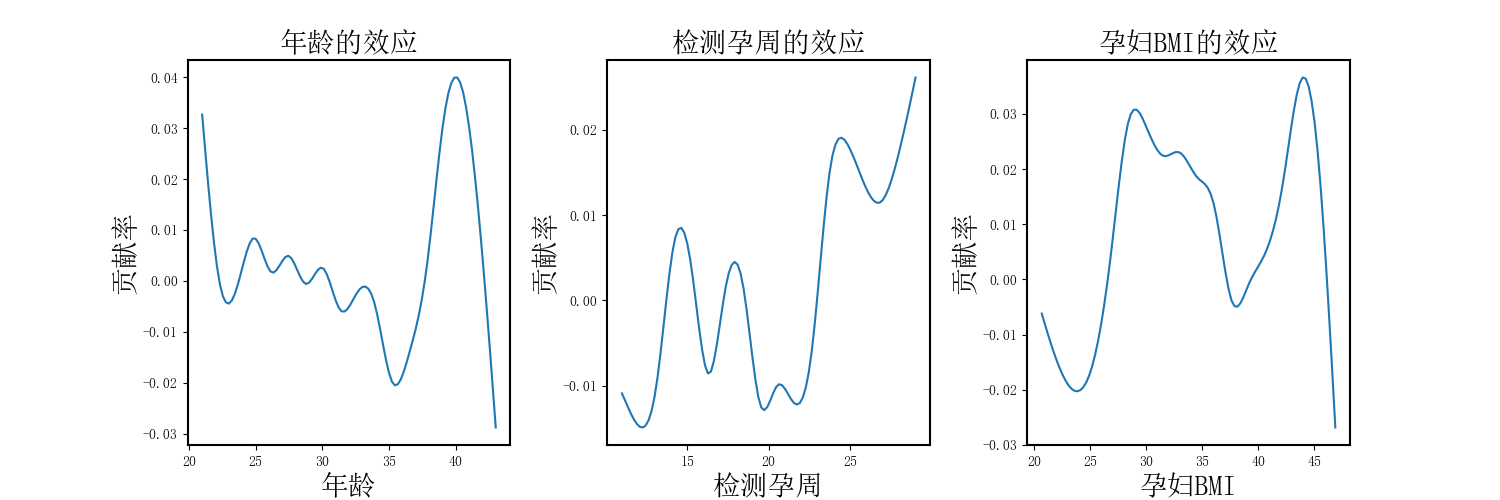
\includegraphics[width=0.98\textwidth]{gam.png} % 图片路径和大小
		\caption{各因素对$Y$染色体浓度的效应}
	\end{figure}
	
	针对\textbf{孕妇年龄}因素;在40岁时,对男胎$Y$染色体浓度具有强促进作用;在35岁以及44岁时,具有较强的的抑制作用;其余时刻保持较为稳定的波动。
	
	针对\textbf{检测孕周}因素,随着检测孕周的增加,效应曲线逐渐上升,尤其在孕周超过22周后贡献显著增强,说明检测孕周越大,$Y$ 染色体浓度越容易达到检测阈值;
	
	针对\textbf{孕妇BMI}因素,效应曲线呈现多峰结构,中等范围的 BMI 对$Y$染色体浓度贡献较高,而在过高或过低的 孕妇BMI 区间均表现为负向贡献。
	
	综上,三项指标对 $Y$ 染色体浓度的作用关系均存在\textbf{复杂的非线性变化规律}。
	
	\subsubsection{模型性能与显著性检验}
	
	传统的 $R^2$ 指标常用于处理连续数据,考虑到本题数据的离散性,因此本文采用\textbf{McFadden 伪$R^2$} (pseudo-$R^2$) 来衡量模型的拟合优度,McFadden 伪$R^2$能够较好地反映模型在引入自变量后相较于空模型在拟合优度上的改善幅度,在离散模型问题中被广泛使用,具有较强的解释力和可比性。
	
	McFadden 的 $R^2$ 定义为:
	\begin{equation}
		R^2_{\text{McFadden}} = 1 - \frac{\ln L_{\text{full}}}{\ln L_{\text{null}}}.
	\end{equation}
\begin{itemize}[noitemsep, topsep=0pt, parsep=0pt, partopsep=0pt, leftmargin=1.5em]
	\item \(\ln L_{\text{full}}\) 表示包含自变量的模型的对数似然;
	\item \(\ln L_{\text{null}}\) 表示仅含截距项(空模型)的对数似然。
\end{itemize}


	
	在该模型的实际应用中,McFadden伪$R^2$ 达到\textbf{0.783},说明GAM 模型相较于空模型在解释因变量变异方面具有显著优势,同时也表示我们的模型在本题中具有较好的拟合效果。
	
	\section{问题二求解}

	\subsection{模型建立}
	考虑到男胎孕妇的BMI是影响胎儿$Y$染色体浓度最早达标时间的重要因素,因此需要对不同BMI的孕妇进行合理分组,最小化NIPT检测风险,以更加符合实际情况。本文通过\textbf{K-Means聚类模型}划分了体质相似的孕妇,并通过建立风险期望模型量化检测风险,并测试不同聚类方案下风险的差异情况。

	\subsubsection{风险评估}
		实际情况下,应尽早发现不健康的胎儿,,否则孕妇将会存在风险,因此我们将风险由低至高量化为0-10的数值类型。\textbf{早期发现(12周以内)}风险较低,定义风险程度为$c_2$;\textbf{中期发现(13-27周)}风险高,定义风险程度为$c_3$;\textbf{晚期(28周以后)}发现风险极高,定义风险程度为$c_4$;同时,由于$Y$染色体浓度必须要达到\textbf{4\%}才能保证NIPT检测结果基本准确,为了避免无意义的损失,我们将\textbf{无效检测}定义风险程度为$c_1$;
		
		本文将各组风险程定量化定义为:
	\[
	C(y,t) =
	\begin{cases}
		c_1, & y < 0.04, \\
		c_2, & y \geq 0.04 , t \textless 12, \\
		c_3, & y \geq 0.04 , 12 \le t \textless 27,\\
		c_4, & y \geq 0.04 ,  t \ge 27.
	\end{cases}
	\quad (c_1 < c_2 < c_3 < c_4)
	\]
	\begin{itemize}[noitemsep, topsep=0pt, parsep=0pt, partopsep=0pt, leftmargin=1.5em]
		\item $y$ 表示孕妇$Y$染色体浓度;
		\item $t$ 表示首次$Y$染色体浓度达到4\%时的检测孕周。
	\end{itemize}
	
	\subsubsection{风险概率建模}
 考虑到所给数据量较大的特点,因此可近似将组内频率视为组内概率,在第$i$组划分中,假设孕妇$Y$染色体浓度为$y$,首次$Y$染色体浓度达到4\%时的检测孕周为$t$,定义:检测无效概率为$p_1$,低风险概率为$p_2$,高风险概率为$p_3$,极高风险概率为$p_4$:
 \[
\begin{cases}
	p_1(i) = \Pr(y < 0.04), \\
	p_2(i) = \Pr(y \geq 0.04   , t \textless 12), \\
	p_3(i) = \Pr(y \geq 0.04   ,12 \le t \textless 27), \\
	p_4(i) = \Pr(y \geq 0.04   , t \ge 27).
\end{cases}
\]
	\begin{itemize}[noitemsep, topsep=0pt, parsep=0pt, partopsep=0pt, leftmargin=1.5em]
		\item $p_1(i)$ 表示在第$i$组划分中,检测无效的概率;
		\item  $p_2(i)$ 表示在第$i$组划分中,孕妇处于低风险的概率;
		\item  $p_3(i)$ 表示在第$i$组划分中,孕妇处于高风险的概率;
		\item  $p_4(i)$ 表示在第$i$组划分中,孕妇处于极高风险的概率。
	\end{itemize}
	
	\subsubsection{分组划分}
	由于BMI是影响胎儿$Y$染色体达标浓度的关键因素,并且它与孕周之间存在复杂的非线性关系,因此常规地依靠经验分组无法充分反应它们之间的内部结构,因此本文选择可解释性强的\textbf{K-means聚类}算法。

K-means 聚类的目标是将 \(n\) 个样本 \(\{x_1, \dots, x_n\}\) 划分为 \(K\) 个簇 \(C = \{C_1, \dots, C_K\}\),以最小化簇内平方误差(Within-Cluster Sum of Squares, WCSS):
	
	\[
	\min_{C_1,\dots,C_K} \;
	J = \sum_{k=1}^K \sum_{x_i \in C_k} \|x_i - \mu_k\|^2.
	\]
	
	其中,\(\mu_k\) 表示第 \(k\) 个簇的质心(centroid),定义为:
	
	\[
	\mu_k = \frac{1}{|C_k|}\sum_{x_i \in C_k} x_i.
	\]
	

	在聚类分析过程中,本文发现影响孕妇最佳NIPT时点的主要因素是个体间生理特征的差异性。为了客观地划分BMI区间,本文将孕妇$Y$染色体浓度首次达到4\%的检测孕周$T$和BMI作为聚类特征进行划分,得到$K$个划分区间。在每个划分区间中,孕妇具有相似的生理特征与达标时间,本文通过这些特征来划分不同的群体,从而为每个簇确定最佳的 NIPT 检测时点。
	
	算法具体步骤如下:
	
		1.\textbf{初始化}:随机选择 \(K\) 个样本点(即选取 \(K\) 个孕妇样本的 BMI 和检测孕周 \(T\))作为初始质心;
		
		2. \textbf{分配}:根据每个孕妇的 BMI 和 $Y$ 染色体浓度首次达到 4\% 的检测孕周,将每个样本 \(x_i = (BMI_i, T_i)\) 分配到最近的质心对应的簇:
		\[
		C_k = \{x_i : \|x_i - \mu_k\|^2 \leq \|x_i - \mu_j\|^2, \;\forall j\}.
		\]
		
		3. \textbf{更新}:根据新的分簇结果,更新每个簇的质心 \(\mu_k\),即更新每个簇内孕妇的 BMI 和检测孕周的均值;
		
		4. \textbf{重复}:重复步骤 2 和 3,直到簇分配不再变化,或者目标函数 \(J\) 收敛。
	
	\subsubsection{量化风险}
 	划分的核心目标在于最小化孕妇群体在接受NIPT检测过程中所面临的潜在风险。为此,本文制定了两点系统性风险优化目标:
	
	(1)孕妇量化风险总和实现最小化,即:
	\begin{equation}
		min\ \frac{1}{K}\sum_{j = 1}^{K} \sum_{i = 1}^{4}c_i \cdot p_i(j)
	\end{equation}
	
	(2)各BMI组间的风险分布应该尽可能均衡,即组间风险离散程度最小化:
	\begin{equation}
		min\ \mathrm{Var}(R) = \frac{1}{K}\sum_{j=1}^K 
		\left(
		\sum_{i=1}^4 c_i \, p_i(j) - 
		\frac{1}{K}\sum_{k=1}^K \sum_{i=1}^4 c_i \, p_i(k)
		\right)^2
	\end{equation}
	\begin{itemize}[noitemsep, topsep=0pt, parsep=0pt, partopsep=0pt, leftmargin=1.5em]
		\item $c_i$ 表示第$i$个风险程度;
		\item $p_i(k)$ 表示第$k$个分组中达到第$i$个风险程度的概率。
	\end{itemize}
	\subsubsection{模型求解}
	为了量化风险程度,本文规定风险程度由低到高依次为为$0\dots10$,即$c_1 = 2,c_2 = 4,c_3 = 6,c_4 = 8$;
	
	同时为了实现系统性风险优化目标,本文根据聚类指标综合划分了\textbf{不同簇数},最终得到了不同划分簇数下风险指标的具体值:
	
	\begin{table}[htbp]
		\centering
		\caption{划分簇数与聚类指标的关系}
		\begin{threeparttable}
			\setlength{\tabcolsep}{6pt} % 减小列数多的表格的列间距
			\small % 为列数多的表格使用稍小的字体
			\begin{tabular}{ c *{5}{c} } % 使用 * 语法简化列格式定义
				\toprule
				聚类指标 & $K = 2$ & $K = 3$ & $K = 4$ & $K = 5$ & $K = 6$ \\
				\midrule
				$\mu$    & 5.7105 & 5.7114 & 5.6468 & 5.6347 & 5.6170 \\
				$\sigma^2$ & 0.0121 & 0.0136 & 0.0497 & 0.0345 & 0.0444 \\
				\bottomrule
			\end{tabular}
		\end{threeparttable}
	\end{table}

	观察结果,当$K=5$的时候,均值和方差均较小,即在系统总风险相对较低的同时,组间风险分布较为均衡,优化效果较好,故选择$K=5$作为K-means聚类的簇数。
	
	将$K=5$代入上述聚类模型求解,得到各组聚类中心,考虑到BMI区间划分应保持简洁易懂的原则,因此本文对求解出的聚类中心进行了向上取整,并将区间边界设置为各聚类中心间的中点。
	
	最终得到最优的 BMI 区间和最佳 NIPT 时点为:
\begin{table}[H]
	\centering
		\caption{孕妇 BMI 区间与最佳 NIPT 时点}
	\begin{threeparttable}
		\setlength{\tabcolsep}{14pt} % 控制列间距
		\begin{tabular}{ccc}
			\toprule
		区间左端点& 区间右端点& 最佳时点\\
			\midrule
			25 & 30 & 12.55 \\
			\bottomrule
		\end{tabular}
	\end{threeparttable}

\end{table}

\begin{table}[htbp]
	\centering
	\begin{threeparttable}
		\setlength{\tabcolsep}{14pt} % 控制列间距
		\begin{tabular}{ccc}
			\toprule
			区间左端点& 区间右端点& 最佳时点\\
			\midrule
						30 & 32 & 18.34 \\
			32 & 35 & 12.63 \\
			35 & 38 & 13.57 \\
			38 & 48 & 22.29 \\
			\bottomrule
		\end{tabular}
	\end{threeparttable}
	
\end{table}


在该区间划分下,总体风险为\textbf{5.6347},为高风险区;考虑到在数据中,大部分产妇检测出$Y$染色体浓度大于0.04时,已处于高风险时间,因此总体风险的\textbf{实际意义较强}。

	\subsection{检测误差的影响}
	通过查阅相关资料。检测误差主要来源于三个核心环节:湿实验(Wet Lab)环节、干实验(Dry Lab)环节和生物学变异环节。同时,检测误差对于结果具有显著影响,具体会体现在对于待测染色体浓度的扰动。
	
	在本文中,为了模拟此扰动,我们对$Y$染色体浓度引入了\textbf{高斯白噪声},高斯白噪声不仅能够刻画出检测过程中不可避免的随机误差,而且具有较好的独立性与可解析性。
	
	假设观测到的 $Y$ 染色体浓度 
	$\tilde{Y}(t)$ 由真实浓度 $Y(t)$ 与测量噪声 $\varepsilon_t$ 叠加而成:
	\begin{equation}
	\tilde{Y}(t) = Y(t) + \varepsilon_t,
	\end{equation}
	其中噪声项 $\varepsilon_t$ 被建模为高斯白噪声,即
	\begin{equation}
	\varepsilon_t \sim \mathcal{N}(0,\sigma^2), \qquad
	\mathrm{Cov}(\varepsilon_t,\varepsilon_s) = 
	\begin{cases}
		\sigma^2, & t=s, \\
		0, & t\neq s.
	\end{cases}
	\end{equation}
	
	使用经过高斯白噪声扰动的$Y$染色体浓度数据进行K次以(T,BMI)为标准的\textbf{PE-K-means模型}求解,得到K个聚簇中心 $\{\mu_1,\mu_2,\dots,\mu_K\}$,
	其中 $\mu_k=(\overline{\mathrm{BMI}}_k,\; \overline{T}_k)^\top$ 表示第 $k$ 个簇的平均体质指数
	与平均首次达标孕周。同时,每个簇对应一个最优 NIPT 时点 $t_k^*$。
	据此,构造二维样本点集合
	\[
	x_k = \begin{bmatrix} \overline{T}_k \\[2pt] t_k^* \end{bmatrix},
	\qquad k=1,2,\dots,K
	\]
	
	将使用高斯白噪声构造好的二维样本点集合使用模型重新求解,并将此过程重复1000次,得到以下结果图:
	\begin{figure}[H]
		\centering
		% 第一行
		\subfigure[BMI中心变化]{\includegraphics[width=0.45\textwidth]{Q2e.png}}
		\subfigure[BMI中心箱线图]{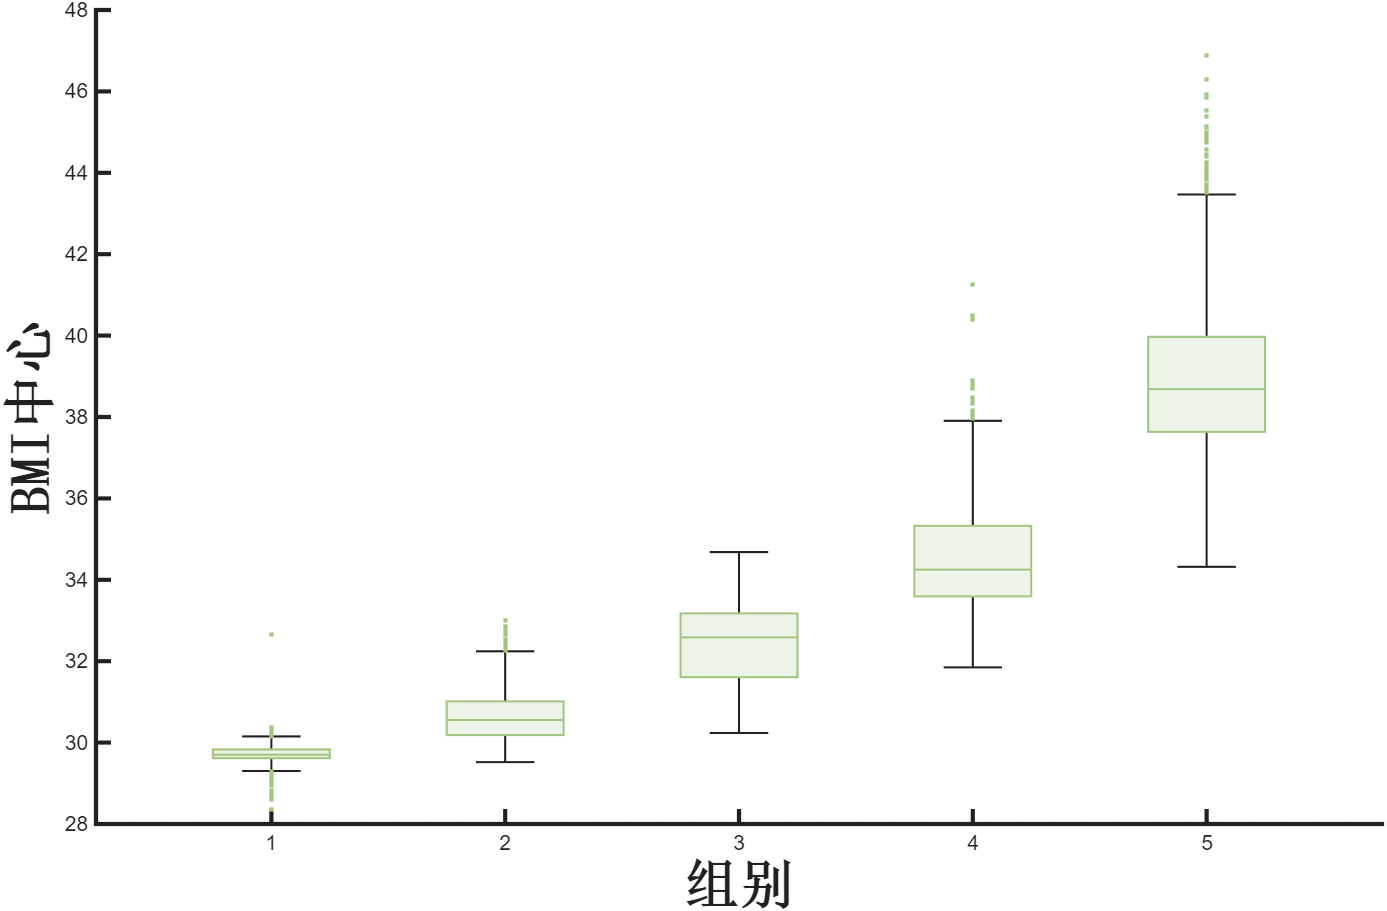
\includegraphics[width=0.45\textwidth]{q2xx.png}}
		\caption{高斯白噪声扰动结果}
		\label{q2e}
	\end{figure}
	
	为评估模型抗干扰能力,我们进行了1000次高斯白噪声扰动模拟。如图\ref{q2e}所示,各聚类中心的BMI估计值波动轻微。该结果从统计学角度证实,在预期\textbf{80\%置信水平}内波动幅度较小,聚类中心的\textbf{方差为1.6159},表明模型的核心参数估计具有高度的稳定性,保证了其在真实场景下的可靠性。
	
	\section{问题三求解}

	\subsection{模型建立}
	\subsubsection{共线性诊断}
	BMI作为身高和体重的衍生指标,其与源变量间必然存在数学上的确定性关系。为在统计分析中避免由此引发的多重共线性问题,并验证使用BMI单一指标的有效性,本研究进行了\textbf{方差膨胀因子(VIF)}诊断。
	\begin{table}[htbp]
		\centering
				\caption{共线性诊断}
		\setlength{\tabcolsep}{23pt} % 控制列间距
		\begin{tabular}{ccc}
			\toprule
			维度 & 特征值 & 条件指标 \\
			\midrule
			BMI & 2.992 & 1.000 \\
			身高 & 0.008 & 19.382 \\
			体重 & 0.000 & 89.221 \\
			\bottomrule
		\end{tabular}
	\end{table}
	
	结果表明BMI与身高体重的方差膨胀因子分别为19.32与89.221,因此具有较强的\textbf{共线性},所以本文使用可使用BMI代替身高体重作为影响$Y$染色体浓度达标时间的主要因素之一。
	
	\subsubsection{相关性判断}
	
	为了探索与检测孕周相关的多种\textbf{非线性}因素,本文题沿用问题一中的\textbf{spearman相关系数},得到结果如下:
	\begin{table}[H]
		\centering
		\caption{斯皮尔曼相关系数矩阵}
		\begin{threeparttable}
			\setlength{\tabcolsep}{5pt} % 调整列间距
			\begin{tabular}{lcccc} 
				\toprule
				& $Y$染色体浓度 & 孕妇年龄  & 孕妇BMI  & 生产次数 \\
				\cmidrule(lr){2-5}
				相关系数
				& 0.84 & $0.064$ & $0.137$ &  $0.000$  \\
				显著性(双尾)
				& 0.006 & $0.037$ & <0.001 & $0.991$   \\
				N
				& 1082 & 1082 & 1082 & 1082  \\
				\bottomrule
			\end{tabular}
		\end{threeparttable}
	\end{table}

	根据假设检验,在显著性水平为1\%时,检测孕周与孕妇BMI和$Y$染色体浓度具有较强的相关性,显著性水平度为5\%时,检测孕周与孕妇年龄具有较强的相关性。
	
	\subsubsection{孕周预测模型}
	孕妇BMI、孕妇年龄、检测孕周以及$Y$染色体浓度之间存在复杂的\textbf{非线性}关系,本文采用对非线性拟合性较好的\textbf{广义加性模型(GAM)},该模型能够通过平滑函数灵活地拟合每个自变量(BMI、年龄、检测孕周)与因变量($Y$染色体浓度)之间的非线性响应,从而建立更为精确和稳健的关联模型。
	
	设响应变量为 $T$(表示检测孕周),自变量为
	$X_1 = \text{年龄},
	X_2 = \text{Y染色体浓度}, 
	X_3 = \text{孕妇BMI}$。
	则广义加性模型 (Generalized Additive Model, GAM)可表示为:
	\begin{equation}
		T
		= \beta_0 + f_1(X_1) + f_2(X_2) + f_3(X_3).
	\end{equation}
	其中:
	$\beta_0$ 为截距项;$f_1(\cdot), f_2(\cdot), f_3(\cdot)$ 分别用于刻画 $X_1, X_2, X_3$ 对 $T$ 的影响力。
	
	具体而言,每个平滑函数可展开为样条基函数的线性组合:
	\begin{equation}
		f_j(x) = \sum_{k=1}^{K_j} \beta_{jk}\, b_{jk}(x), \quad j=1,2,3.
	\end{equation}
	其中 $b_{jk}(x)$ 为样条基函数,$\beta_{jk}$ 为待估参数。
	参数通过最大化惩罚似然得到:
	\begin{equation}
		\ell(\beta) - \sum_{j=1}^3 \lambda_j \int \left(f_j''(x)\right)^2 \, dx.
	\end{equation}
	其中 $\ell(\beta)$ 为似然函数,$\lambda_j$ 为平滑参数。
	
	将“Q1data1.xlsx”数据代入求解,得到拟合完成的检测孕周预测模型。
	\subsubsection{估计临界值数据}
	问题要求孕妇潜在风险要尽可能小,那么对于孕妇来说,越早进行准确的NIPT检测越好,因此$Y$染色体浓度第一次达标的时点是进行NIPT的最佳时点,于是本文对问题一中的模型进行改进得到了检测孕周的预测模型,以此来估计每对BMI年龄(BMI,Age)$Y$染色体浓度第一次达标的时点。
	
	保持附件中每一项数据的BMI和年龄(Age)不变,将0.04代入$Y$染色体浓度并将这组新变量值代入到检测孕周预测模型中,得到了每对(BMI,Age)所对应的第一次$Y$染色体浓度达到4\%的检测孕周时点,部分结果如下图所示:
	\begin{table}[htpb]
		\centering
		\caption{部分预测数据}
		\setlength{\tabcolsep}{14pt}
		\begin{tabular}{lcc}
			\toprule
			年龄 & 孕妇BMI & 预测的检测孕周 \\
			\midrule
			31 & 28.12 & 15.33 \\
			31 & 28.52 & 15.05 \\
			31 & 28.52 & 15.05 \\
			31 & 28.91 & 14.99 \\
			32 & 33.33 & 15.81 \\
			32 & 34.23 & 16.24 \\
			32 & 33.78 & 15.93 \\
			32 & 34.23 & 16.24 \\
			\bottomrule
		\end{tabular}
	\end{table}
	
	详细数据可查看附件“Q3data.xlsx”。
	
	结果显示,相比第二问中的预测最佳NIPT点,波动范围显著降低,,收敛性更强,这表明引入多种变量提高了结果的稳健性。
	\subsubsection{聚簇分组}
	由于BMI是影响孕妇最佳NIPT检测时点的关键因素,并且它与检测孕周和年龄之间存在复杂的\textbf{非线性}关系,同样的,常规地依靠经验分组无法充分反应它们之间的内部结构,因此本题采用第二问中所采用的可解释性强的\textbf{K-means聚类}算法。
	
	K-Means 聚类的目标是将 \(n\) 个样本 \(\{x_1, \dots, x_n\}\) 划分为 \(K\) 个簇 \(C = \{C_1, \dots, C_K\}\),以最小化簇内平方误差(Within-Cluster Sum of Squares, WCSS):
	
	\[
	\min_{C_1,\dots,C_K} \;
	J = \sum_{k=1}^K \sum_{x_i \in C_k} \|x_i - \mu_k\|^2
	\]
	
	其中,\(\mu_k\) 表示第 \(k\) 个簇的质心(centroid),定义为:
	
	\[
	\mu_k = \frac{1}{|C_k|}\sum_{x_i \in C_k} x_i
	\]
	
	
	在聚类分析过程中,为了使得各组内孕妇的最佳NIPT时点尽可能相似,本题将(年龄,BMI,预测的检测孕周)所构成的三元组作为聚类特征进行划分,得到$K$个划分区间。在每个划分区间中,孕妇具有相似的生理特征与达标时间,本文通过这些特征来划分不同的群体,从而为每个簇确定最佳的 NIPT 检测时点。
	
	算法具体步骤如下:
	
	1.\textbf{初始化}:随机选择 \(K\) 个样本点(即选取 \(K\) 个孕妇样本的年龄\(Age\)、BMI 和预测检测孕周 \(T\))作为初始质心;
	
	2. \textbf{分配}:根据每个孕妇的 年龄、BMI 和 预测检测孕周,将每个样本 \(x_i = (Age_i,BMI_i, T_i)\) 分配到最近的质心对应的簇:
	\[
	C_k = \{x_i : \|x_i - \mu_k\|^2 \leq \|x_i - \mu_j\|^2, \;\forall j\}
	\]
	
	3. \textbf{更新}:根据新的分簇结果,更新每个簇的质心 \(\mu_k\),即更新每个簇内孕妇的年龄、 BMI 和检测孕周的均值;
	
	4. \textbf{重复}:重复步骤 2 和 3,直到簇分配不再变化,或者目标函数 \(J\) 收敛。
	
	\subsubsection{风险模型}
	
	划分的核心目标在于最小化孕妇群体在接受NIPT检测过程中所面临的潜在风险。为此,本题沿用第二问中的风险优化目标:
	
	(1)孕妇量化风险总和实现最小化,即:
	\begin{equation}
		min\ \frac{1}{K}\sum_{j = 1}^{K} \sum_{i = 1}^{4}c_i \cdot p_i(j)
	\end{equation}
	其中:
	\[
	C(y,t) =
	\begin{cases}
		c_1, & y < 0.04, \\
		c_2, & y \geq 0.04 , t \textless 12, \\
		c_3, & y \geq 0.04 , 12 \le t \textless 27,\\
		c_4, & y \geq 0.04 ,  t \ge 27.
	\end{cases}
	\quad (c_1 < c_2 < c_3 < c_4)
	\]
	\begin{itemize}[noitemsep, topsep=0pt, parsep=0pt, partopsep=0pt, leftmargin=1.5em]
		\item $c_1$ 表示无效检测;
		\item $c_2$ 表示早期发现(12周以内)的低风险;
		\item $c_3$ 表示中期发现(13-27周)的高风险;
		\item $c_3$ 表示中期发现(13-27周)的高风险;
		\item $y$ 表示晚期(28周以后)发现风险极高;
		\item $t$ 表示首次$Y$染色体浓度达到4\%时的检测孕周。
	\end{itemize}
	
	(2)各BMI组间的风险分布应该尽可能均衡,即组间风险离散程度最小化:
	\begin{equation}
		min\ \mathrm{Var}(R) = \frac{1}{K}\sum_{j=1}^K 
		\left(
		\sum_{i=1}^4 c_i \, p_i(j) - 
		\frac{1}{K}\sum_{k=1}^K \sum_{i=1}^4 c_i \, p_i(k)
		\right)^2
	\end{equation}
	\begin{itemize}[noitemsep, topsep=0pt, parsep=0pt, partopsep=0pt, leftmargin=1.5em]
		\item $c_i$ 表示第$i$个风险程度;
		\item $p_i(k)$ 表示第$k$个分组中达到第$i$个风险程度的概率。
	\end{itemize}
	其中: \[
	\begin{cases}
		p_1(i) = \Pr(y < 0.04), \quad &\text{(无效检测概率)}\\
		p_2(i) = \Pr(y \geq 0.04   , t \textless 12) ,\quad &\text{(低风险概率)}\\
		p_3(i) = \Pr(y \geq 0.04   ,12 \le t \textless 27), \quad &\text{(高风险概率)}\\
		p_4(i) = \Pr(y \geq 0.04   , t \ge 27).\quad &\text{(极高风险概率)}
	\end{cases}
	\]
	
	\subsection{模型求解}
	本题风险程度的量化参照第二问中定义的等级系数,即:$c_1 = 2$(低风险),$c_2 = 4$(中风险),$c_3 = 6$(高风险),$c_4 = 8$(较高风险);
	

	为实现系统性风险最小化的目标,本文基于聚类指标对不同分组数量(簇数)进行了综合评估。通过比较不同簇数划分方案下的系统风险期望,最终确定了最优分组策略。不同簇数划分下对应的系统风险指标如下表所示:
	
	\begin{table}[htbp]
		\centering
		\caption{划分簇数与聚类指标的关系}
		\begin{threeparttable}
			\setlength{\tabcolsep}{6pt} % 减小列数多的表格的列间距
			\small % 为列数多的表格使用稍小的字体
			\begin{tabular}{ c *{5}{c} } % 使用 * 语法简化列格式定义
				\toprule
				聚类指标 & $K = 2$ & $K = 3$ & $K = 4$ & $K = 5$ & $K = 6$ \\
				\midrule
				$\mu$    & 5.7096 & 5.7135 & 5.7102 & 5.6638 & 5.7006 \\
				$\sigma^2$ & 0.0139 & 0.0157 & 0.0212 & 0.0261 & 0.0350 \\
				\bottomrule
			\end{tabular}
		\end{threeparttable}
	\end{table}
	
	观察结果,当$K=5$的时候,均值较小且方差在可接受范围内,即在系统总风险相对较低的同时,组间风险分布较为均衡,优化效果较好,故选择$K=5$作为K-means聚类的簇数。
	
	值得注意的是,相较于问题二,当引入了\textbf{孕妇年龄}等更多的相关变量以及\textbf{预测的$Y$染色体浓度首次达标时点},在总体风险程度相近的情况下,\textbf{方差更小},证明分组更加合理。
	
	将$K=5$代入上述聚类模型求解,得到各组聚类中心,并将其向上取整,将区间边界设置为各聚类中心间的中点。
	
	最终得到最优的 BMI 区间和最佳 NIPT 时点为:
	\begin{table}[htbp]
		\centering
		\caption{孕妇 BMI 区间与最佳 NIPT 时点}
		\begin{threeparttable}
			\setlength{\tabcolsep}{14pt} % 控制列间距
			\begin{tabular}{ccc}
				\toprule
				区间左端点& 区间右端点& 最佳时点\\
				\midrule
				25 & 31 & 15.57 \\
				31 & 32 & 15.93 \\
				32 & 33 & 16.22 \\
				33 & 36 & 15.87 \\
				36 & 48 & 18.38 \\
				\bottomrule
			\end{tabular}
		\end{threeparttable}
	\end{table}
	
	在该区间划分下,总体风险为5.6638,为高风险区;相较于第二问中划分的BMI区间风险期望均值略有降低。
	
	较于问题二所构建的模型,本题建立的模型综合考虑了\textbf{孕妇身高、体重、年龄、BMI、$Y$染色体浓度}等多种因素,所得到的依据孕妇BMI划分的区间更具合理性,同时各组最佳时点的\textbf{离散程度}有\textbf{显著降低},并且检测时点普遍\textbf{较早},从而降低了孕妇在整个孕期内可能面临的潜在风险。
	
	\subsection{检测误差的影响}
	检测的误差主要体现在$Y$染色体浓度的误差上,从而导致后续求解出现波动。为了评价在有检测误差的前提下模型的表现如何,本题对$Y$染色体浓度引入具有较好独立性的\textbf{高斯白噪声}扰动。
	
	假设观测到的 $Y$ 染色体浓度 
	$\tilde{Y}(t)$ 由真实浓度 $Y(t)$ 与测量噪声 $\varepsilon_t$ 叠加而成:
	\begin{equation}
		\tilde{Y}(t) = Y(t) + \varepsilon_t.
	\end{equation}
	其中噪声项 $\varepsilon_t$ 被建模为高斯白噪声,即
	\begin{equation}
		\varepsilon_t \sim \mathcal{N}(0,\sigma^2), \qquad
		\mathrm{Cov}(\varepsilon_t,\varepsilon_s) = 
		\begin{cases}
			\sigma^2, & t=s, \\
			0, & t\neq s.
		\end{cases}
	\end{equation}
	
	使用经过高斯白噪声扰动的$Y$染色体浓度数据进行K次以(Age,BMI,T)为标准的PE-K-means模型求解,得到K个聚簇中心 $\{\mu_1,\mu_2,\dots,\mu_K\}$,
	其中 $\mu_k=(\overline{\mathrm{Age}}_k,\;\overline{\mathrm{BMI}}_k,\; \overline{T}_k)^\top$ 表示第 $k$ 个簇的平均年龄、平均BMI
	与平均首次达标孕周。同时,每个簇对应一个最优 NIPT 时点 $t_k^*$。
	据此,构造三维样本点集合
	\[
	x_k = \begin{bmatrix} \overline{T}_k \\[2pt] t_k^* \end{bmatrix},
	\qquad k=1,2,\dots,K
	\]
	
	将使用高斯白噪声构造好的二维样本点集合使用模型重新求解,并将此过程重复1000次,得到以下结果图:
\begin{figure}[htbp]
	\centering
	% 第一行
	\subfigure[BMI中心变化]{\includegraphics[width=0.45\textwidth]{Q3e.png}}
	\subfigure[BMI中心箱线图]{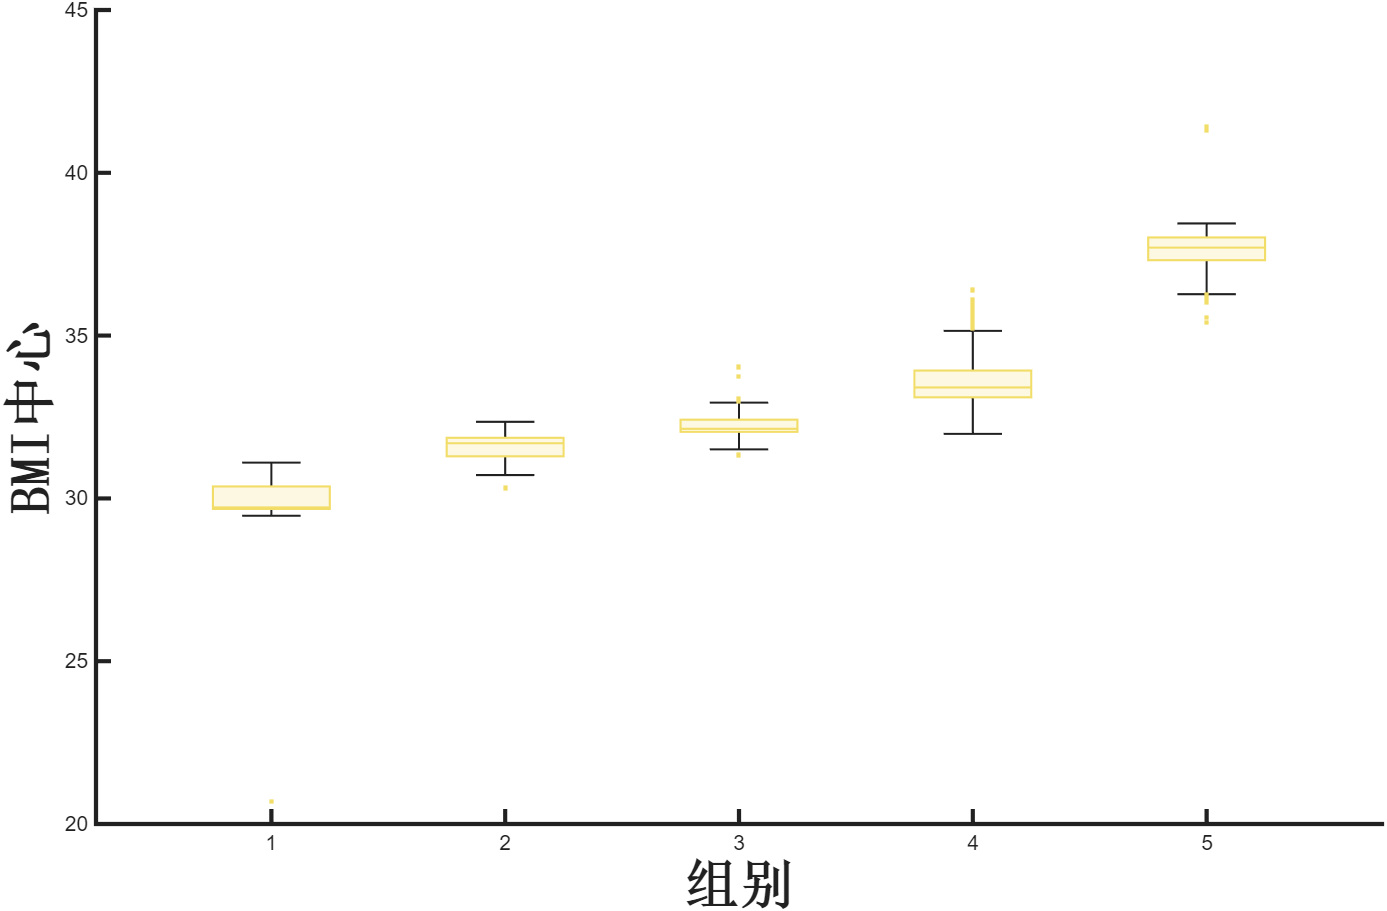
\includegraphics[width=0.45\textwidth]{q3xx.png}}
	\caption{高斯白噪声扰动结果}
\end{figure}
	
	根据图像所示,在1000次随机高斯白噪声的扰动下,聚类中心方差为0.4188,相较于问题二呈现出更为显著的稳定性,其波动大部分局限在极小的范围内。证明综合考虑了\textbf{孕妇身高、体重、年龄、BMI、$Y$染色体浓度}等因素后,BMI中心箱线图较于问题二,数据不仅更加集中,而且离群值大幅度减少,这说明综合考虑多种变量因素的改善PE-K-means模型具有更为优异的鲁棒性,所求的区间也更为实际、合理。
	
	\section{问题四求解}
	
	\subsection{数据预处理}
	
	NIPT检测通过检测胎儿21、18、13号染色体是否具有非整倍性异常来判断胎儿是否健康。因此,本文将问题拆分为三个独立的二分类目标,即分别判断21号染色体、18号染色体和13号染色体是否异常。在NIPT检测中,对于常见染色体非整倍体检测,通常采用 Z 值分析方法进行统计判定,且每条染色体所采集到的读段数量与该染色体长度成正比。由此可知21、18、13号染色体是否异常与各自的染色体Z值、GC含量有着密切关系,同时也与读段数量、GC含量以及BMI有关。
	
	本文首先分别提取21号、18号和13号染色体异常的和正常样本的相关特征数据。随后,结合无异常数据与各组异常数据进行数据\textbf{归一化处理},,消除量纲的影响,从而得到了三组标准化的数据集,为后续建模打下基础。
	
	\subsection{模型建立与求解}
	
	本题中,数据是由多个特征组成的样本数据 \( X = \{x_1, x_2, \dots, x_n\} \),其中每个样本 \( x_i \in \mathbb{R}^d \) 是一个 \( d \)-维的特征向量,且对应的标签为 \( y_i \in \{0, 1\} \),表示该样本是否是某种染色体异常。
	
	通过观察附件发现异常样本只占样本总数的10\%,样本极其\textbf{不平衡}。模型的目标是基于这些特征预测每个样本的标签,考虑到在类别不平衡的情况下,\textbf{带L2正则化的逻辑回归模型}具有良好的分类效果,因此我们根据所给数据建立逻辑回归模型。
	
	逻辑回归模型的目标是找到一个线性函数,通过该函数将输入特征 \( x_i \) 映射到输出概率值,其数学表达式为:
	
	\begin{equation}
	P(y_i = 1 | x_i) = \sigma(\mathbf{w}^T x_i + b)
	\end{equation}
	
	其中,\( \sigma(z) = \frac{1}{1 + e^{-z}} \) 为Sigmoid函数,\( \mathbf{w} \in \mathbb{R}^d \) 是模型的权重向量,\( b \in \mathbb{R} \) 是偏置项。目标是通过训练数据优化参数 \( \mathbf{w} \) 和 \( b \),使得模型能够准确地预测样本 \( x_i \) 属于类别 1 的概率。
	
	由于异常样本较少,为了防止过拟合,本文在损失函数中引入了L2正则化项,的目标是约束模型权重的大小,从而提高模型的泛化能力。带L2正则化的逻辑回归损失函数为:
	
	\[
	L(\mathbf{w}, b) = -\sum_{i=1}^{n} \left[ y_i \log(\sigma(\mathbf{w}^T x_i + b)) + (1 - y_i) \log(1 - \sigma(\mathbf{w}^T x_i + b)) \right] + \lambda \|\mathbf{w}\|^2
	\]
	
	其中,\( \lambda \) 是正则化系数,控制L2正则化的强度。通过最小化上述损失函数,可以得到最优的模型参数 \( \mathbf{w} \) 和 \( b \)。将样本数据划分为70\%的训练集和30\%的测试集,训练集用于训练模型,测试集用于模型预测,并评估模型性能。
	
	\subsection{模型评估}
	
	为了评估模型的性能,本文采用的评估指标为\textbf{准确率(Accuracy)}:
	\begin{equation}
	\text{Accuracy} = \frac{TP + TN}{TP + TN + FP + FN}
	\end{equation}
	
	其中:
	\begin{itemize}[noitemsep, topsep=0pt, parsep=0pt, partopsep=0pt, leftmargin=1.5em]
		\item \( TP \) 为真正例(True Positive):模型正确预测为正例的样本数。
		\item \( TN \) 为真负例(True Negative):模型正确预测为负例的样本数。
		\item \( FP \) 为假正例(False Positive):模型错误地将负例预测为正例的样本数。
		\item \( FN \) 为假负例(False Negative):模型错误地将正例预测为负例的样本数。
	\end{itemize}
		
	
	每条染色体的准确率如下所示:
\begin{table}[htbp]
	\centering
	\caption{孕妇 BMI 区间与最佳 NIPT 时点}
	\begin{threeparttable}
		\setlength{\tabcolsep}{12pt} % 可根据实际宽度适当调整间距
		\begin{tabular}{cccc}
			\toprule
			\textbf{染色体编号} & \textbf{准确率} & \textbf{召回率} & \textbf{平均精确度} \\
			\midrule
			13号染色体 & 95.05\% & 4.59\% & 92.30\% \\
			18号染色体 & 90.11\% & 16.36\% & 89.75\% \\
			21号染色体 & 97.25\% & 2.75\% & 96.80\% \\
			\bottomrule
		\end{tabular}
	\end{threeparttable}
\end{table}
	
	在综合考虑了目标染色体的Z值和GC含量、孕妇BMI、读段数及相关比例等因素后,模型对于三种目标染色体的异常判断有着极高的准确性,诊断结果可信度较高。并且在实际情况的大样本量中,由于数据异常样本较多,我们的召回率将会显著升高,因此我们的模型具有良好的拓展性,具备处理复杂情况的潜力。
	
	\section{模型的评价与改进}
	\subsection{模型的优点}
	
(1)本文首先通过共线性检测与相关性分析,在建模过程中选择性地采用特征,保证了数据质量;随后基于孕妇BMI、年龄、$Y$染色体浓度等关键因素,结合聚类算法与统计建模方法,构建了对孕妇群体进行科学分组的综合评价体系,既简化了问题复杂度,又实现了对群体特征的合理刻画。

(2)本文针对不同类别的孕妇群体,通过散点图、拟合曲线、置信区间段多种可视化方式,全面展示了$Y$染色体浓度随孕周、BMI等变量的变化规律,并依据其变化特征将群体划分为稳定达标型、缓慢增长型、波动型等类别,分别采用广义加性模型(GAM)、回归分析等方法对其最佳NIPT时点进行预测,预测结果稳健且贴合临床实际。

(3)本文建立了风险量化模型,将不同发现时点与风险等级相关联,使用数学期望的概念构建以“潜在风险最小”为目标的优化模型,使最佳时点的判定不仅依赖于统计学规律,还具备明确的临床意义,增强了模型的实用性与解释性。

(4)本文引入高斯白噪声模拟检测误差,对模型进行鲁棒性检验,结果表明在不同噪声水平下模型输出保持稳定,进一步验证了所提方法在真实场景中的可靠性与适应性。
	
	\subsection{模型的缺点}
	(1)因为样本量较小的特点,将频率当作概率可能不能完美还原现实情况。
	
	(2)对$X$染色体及上述染色体的 Z 值、GC含量、读段数及相关比例、BMI 等影响因素可解释性较弱,仅仅从预测精度上进行了拟合优化。
	\subsection{模型的推广}
	本文建立的模型可广泛应用于NIPT检测的风险评估、对于未来数据的预测、对货物的订购与转运计划等问题,实用性强,可推广性高。
	
	\newpage
	\begin{thebibliography}{9}
		%\section*{参考文献}
		\bibitem[1]{wang2013} Wang E, Batey A, Struble C, Musci T, Song K, Oliphant A. Gestational age and maternal weight effects on fetal cell-free DNA in maternal plasma[J]. Prenatal Diagnosis, 2013, 33(7): 662–666. DOI: 10.1002/pd.4119.
		
		\bibitem[2]{canick} Canick J A, Palomaki G E, Kloza E M, Lambert\textendash Messerlian G M, Haddow J E. The impact of maternal plasma DNA fetal fraction on next generation sequencing tests for common fetal aneuploidies[J]. Prenatal Diagnosis, 2013: Early View. DOI: 10.1002/pd.4126.
		
		\bibitem[3]{deepseek}DeepSeek, DeepSeek-V3.1, 深度求索(DeepSeek), 2025-09-06.
		\bibitem[4]{deepseek}DeepSeek, DeepSeek-V3.1, 深度求索(DeepSeek), 2025-09-07.
		
	\end{thebibliography}
	
	\newpage
	\section*{附录}
	\subsection*{附录1 源程序列表}
		\begin{itemize}[noitemsep, topsep=0pt, parsep=0pt, partopsep=0pt, leftmargin=1.5em]
		\item Q1dp.m
		\item Q1BMI.m
		\item Q1ga.m
		\item age.m
		\item gam.py
		\item Q2.m
		\item Q2e.m
		\item Q3gam.py
		\item Q3.m
		\item Q3game.py
		\item Q3e.m
		\item Q4.py
	\end{itemize}
\subsection*{附录2 支撑数据及图片列表}
\begin{itemize}[noitemsep, topsep=0pt, parsep=0pt, partopsep=0pt, leftmargin=1.5em]
	\item age.png
	\item age.xlsx
	\item BMI27-30.png
	\item BMI30-33.png
	\item BMI33-36.png
	\item BMI36-39.png
	\item BMI27-30.xlsx
	\item BMI30-33.xlsx
	\item BMI33-36.xlsx
	\item BMI36-39.xlsx
	\item ga11-14.png
	\item ga14-17.png
	\item ga17-20.png
	\item ga20-23.png
	\item ga11-14.xlsx
	\item ga14-17.xlsx
	\item ga17-20.xlsx
	\item ga20-23.xlsx
	\item Q1data.xlsx
	\item Q1lc.png
	\item q2e.png
	\item Q2lc.png
	\item q2xx.png
	\item Q3data.xlsx
	\item Q3datae.xlsx
	\item q3e.png
	\item Q3lc.png
	\item q3xx.png
	\item Q4lc.png
	\item 附件.xlsx
	\item AI工具使用详情.pdf
\end{itemize}
	\subsection*{附录3 源程序代码}

	\noindent \textbf{\heiti 1.问题一数据预处理代码(Q1dp.m)}
	\begin{verbatim}
		clc,clear
		data=readcell('附件.xlsx');
		%将附件中序号为209的检测孕周中的“16W+1”改为“16w+1”
		colind=[3,10,11,22];
		data=data(2:end,colind);
		for i=1:size(data,1)
		converted_str = strrep(data{i,2}, 'w', '*7');
		data{i,2}=eval(converted_str)/7;
		end
		data=cell2mat(data);
		writematrix(data,'Q1data.xlsx')
	\end{verbatim}
	\noindent \textbf{\heiti 2.问题一$Y$染色体浓度与孕妇BMI散点图绘制代码(Q1BMI.m)}
	\begin{verbatim}
		clc,clear
		data=readmatrix('Q1data.xlsx');
		data=data(data(:,1)==28,2:end);
		data1=data(data(:,1)>=11&data(:,1)<14,:);
		data2=data(data(:,1)>=14&data(:,1)<17,:);
		data3=data(data(:,1)>=17&data(:,1)<20,:);
		data4=data(data(:,1)>=20&data(:,1)<23,:);
		
		figure
		scatter(data1(:,2),data1(:,3),50,'r','filled')
		xlabel('孕妇BMI/(kg/m^2)','Interpreter','tex')
		ylabel('Y染色体浓度/(%)')
		writematrix(data1,'BMI27-30.xlsx')
		grid on
		
		figure
		scatter(data2(:,2),data2(:,3),50,'b','filled')
		xlabel('孕妇BMI/(kg/m^2)','Interpreter','tex')
		ylabel('Y染色体浓度/(%)')
		writematrix(data2,'BMI30-33.xlsx')
		grid on
		
		figure
		scatter(data3(:,2),data3(:,3),50,[0.9, 0.4, 0],'filled')
		xlabel('孕妇BMI/(kg/m^2)','Interpreter','tex')
		ylabel('Y染色体浓度/(%)')
		writematrix(data3,'BMI33-36.xlsx')
		grid on
		
		figure
		scatter(data4(:,2),data4(:,3),50,[0, 0.7, 0.9],'filled')
		xlabel('孕妇BMI/(kg/m^2)','Interpreter','tex')
		ylabel('Y染色体浓度/(%)')
		writematrix(data4,'BMI36-39.xlsx')
		grid on
	\end{verbatim}
	\noindent \textbf{\heiti 3.问题一Y染色体浓度与检测孕周散点图绘制代码(Q1ga.m)}
	\begin{verbatim}
		clc,clear
		data=readmatrix('Q1data.xlsx');
		data=data(data(:,1)==28,2:end);
		data1=data(data(:,2)>=27&data(:,2)<30,:);
		data2=data(data(:,2)>=30&data(:,2)<33,:);
		data3=data(data(:,2)>=33&data(:,2)<36,:);
		data4=data(data(:,2)>=36&data(:,2)<39,:);
		
		figure
		scatter(data1(:,1),data1(:,3),50,'r','filled')
		xlabel('检测孕周/(周)')
		ylabel('C')
		writematrix(data1,' ga11-14.xlsx')
		grid on
		
		figure
		scatter(data2(:,1),data2(:,3),50,'b','filled')
		xlabel('检测孕周/(周)')
		ylabel('Y染色体浓度/(%)')
		writematrix(data2,' ga14-17.xlsx')
		grid on
		
		figure
		scatter(data3(:,1),data3(:,3),50,[0.9, 0.4, 0],'filled')
		xlabel('检测孕周/(周)')
		ylabel('Y染色体浓度/(%)')
		writematrix(data3,' ga17-20.xlsx')
		grid on
		
		figure
		scatter(data4(:,1),data4(:,3),50,[0, 0.7, 0.9],'filled')
		xlabel('检测孕周/(周)')
		ylabel('Y染色体浓度/(%)')
		writematrix(data4,' ga20-23.xlsx')
		grid on
	\end{verbatim}
	\noindent \textbf{\heiti 4.问题一Y染色体浓度与孕妇年龄散点图绘制代码(age.m)}
	\begin{verbatim}
		clc,clear
		data=readmatrix('Q1data.xlsx');
		data=data(:,[1,4]);
		group=findgroups(data(:,1));
		mean=splitapply(@mean,data(:,2),group);
		ug=unique(data(:,1));
		
		figure
		scatter(ug,mean,50,'r','filled')
		xlabel('年龄')
		ylabel('Y染色体浓度/(%)')
		writematrix([ug,mean],'age.xlsx')
		grid on
	\end{verbatim}
	
	\noindent \textbf{\heiti 5.问题一GAM模型求解代码(gam.py)}
	\begin{verbatim}
		import pandas as pd
		import numpy as np
		from pygam import LinearGAM, s
		import matplotlib.pyplot as plt
		
		plt.rcParams['font.sans-serif'] = ['SimHei']  
		plt.rcParams['axes.unicode_minus'] = False
		
		file = "Q1data.xlsx"
		date = pd.read_excel(file, header=None)
		date.columns = ["年龄", "检测孕周", "孕妇BMI", "Y染色体浓度"]
		x = date[["年龄", "检测孕周", "孕妇BMI"]].values
		y = date["Y染色体浓度"].values
		gam = LinearGAM(s(0) + s(1) + s(2)).fit(x, y)
		print("Pseudo R²:", gam.statistics_["pseudo_r2"])
		fig, axs = plt.subplots(1, 3, figsize=(15, 5))
		for i, term in enumerate(["年龄", "检测孕周", "孕妇BMI"]):
		xx = gam.generate_X_grid(term=i)
		axs[i].plot(xx[:, i], gam.partial_dependence(term=i, X=xx))
		axs[i].set_xlabel(term)
		axs[i].set_ylabel("贡献率")
		axs[i].set_title(f"{term}的效应")
		plt.show()
		
	\end{verbatim}
	
	\noindent \textbf{\heiti 6.问题二PE-K-means模型求解代码(Q2.m)}
	\begin{verbatim}
		clc,clear
		data=readcell('附件.xlsx');
		colind=[2,3,10,11,22];
		data=data(2:end,colind);
		for i=1:size(data,1)
		converted_str = strrep(data{i,3}, 'w', '*7');
		data{i,3}=eval(converted_str)/7;
		str=regexprep(data{i,1},'[^0-9]','');
		data{i,1}=str2double(str);
		end
		data=cell2mat(data);
		data=data(:,[1,3,4,5]);
		
		x=[];
		alpha=0.04;
		curid=0;
		for i=1:size(data,1)
		if data(i,1)==curid+1
		curid=curid+1;
		end
		if data(i,1)==curid && data(i,4)>=alpha
		curid=curid+1;
		x=[x;data(i,[2,3])];
		end
		end
		
		lb=25;
		rb=48;
		k=5;
		[index,c]=kmeans(x,k);
		c=sortrows(c,2);
		group=zeros(k,3);
		group(1,:)=[lb,round((c(1,2)+c(2,2))/2),c(1,1)];
		for i=2:k-1
		group(i,:)=[round((c(i-1,2)+c(i,2))/2),round((c(i,2)+c(i+1,2))/2),c(i,1)];
		end
		group(k,:)=[round((c(k-1,2)+c(k,2))/2),rb,c(k,1)];
		
		weight=[2,4,6,8];
		week=[12,27];
		
		fval=zeros(k,2);
		for i=1:size(data,1)
		for j=1:k
		if data(i,3)>=group(j,1) && data(i,3)<group(j,2)
		ind=j;
		break;
		end
		end
		if data(i,4)<alpha
		pos=2;
		elseif group(ind,3)<=week(1)
		pos=1;
		elseif group(ind,3)>week(1) && group(ind,3)<=week(2)
		pos=3;
		else
		pos=4;
		end
		fval(ind,1)=fval(ind,1)+weight(pos);
		fval(ind,2)=fval(ind,2)+1;
		end
		
		f=fval(:,1)./fval(:,2);
		f(isnan(f))=0;
		fmean=mean(f);
		fvar=var(f);
	\end{verbatim}
	
	\noindent \textbf{\heiti 7.问题二高斯白噪声模拟检测误差(Q2e.m)}
	\begin{verbatim}
		clc,clear
		data=readcell('附件.xlsx');
		colind=[2,3,10,11,22];
		data=data(2:end,colind);
		for i=1:size(data,1)
		converted_str = strrep(data{i,3}, 'w', '*7');
		data{i,3}=eval(converted_str)/7;
		str=regexprep(data{i,1},'[^0-9]','');
		data{i,1}=str2double(str);
		end
		data=cell2mat(data);
		data=data(:,[1,3,4,5]);
		
		k=5;
		alpha=0.04;
		rd=1000;
		back=data(:,4);
		cp=zeros(k*rd,2);
		for ri=1:rd
		x=[];
		curid=0;
		data(:,4)=back+normrnd(0,0.1,size(data,1),1);
		for i=1:size(data,1)
		if data(i,1)==curid+1
		curid=curid+1;
		end
		if data(i,1)==curid && data(i,4)>=alpha
		curid=curid+1;
		x=[x;data(i,[2,3])];
		end
		end
		[index,c]=kmeans(x,k);
		c=sortrows(c,2);
		c=[c(:,2),c(:,1)];
		cp((ri-1)*k+1:ri*k,:)=c;
		end
		cp(cp(:,1)<=25)=cp(cp(:,1)<=25)+9;
		
		figure
		color={[214 207 103]/256,[104 180 206]/256,[249 156 66]/256,[70 96 173]/256,[0 0 139]/256};
		for i=1:5
		scatter(1:rd,cp(i:5:end,1),10,color{i},'filled')
		hold on
		
		clevel=0.95;
		a=1-clevel;
		fd=rd-1;
		t=tinv(1-a/2,fd);
		me=mean(cp(i:5:end,1));
		SE=me/sqrt(rd);
		CI=t*SE;
		lb=me-CI;
		ub=me+CI;
		
		h=fill([1,rd,rd,1],[ub,ub,lb,lb],color{i},'LineStyle','none');
		set(h,'facealpha',0.2);
		
		plot(1:rd,ones(1,rd)*me,'Color',color{i},'LineWidth',2)
		end
		xlabel('次数')
		ylabel('BMI中心')
		ylim([28,40])
		
		figure
		boxm=[];
		for i=1:5
		boxm=[boxm,cp(i:5:end,1)];
		end
		h=boxchart(boxm);
		h.MarkerStyle='.';
		h.MarkerColor=[165 198 130]/256;
		h.BoxFaceColor=[165 198 130]/256;
		xlabel('组别')
		ylabel('BMI中心')
		
		v=0;
		for i=1:5
		v=v+var(cp(i:5:end,1));
		end
		v=v/5;
	\end{verbatim}
	
		\noindent \textbf{\heiti 8.问题三GAM模型预测检测孕周(Q3gam.py)}
	\begin{verbatim}
		import pandas as pd
		import numpy as np
		from pygam import LinearGAM, s
		import matplotlib.pyplot as plt
		
		plt.rcParams['font.sans-serif'] = ['SimHei']  
		plt.rcParams['axes.unicode_minus'] = False
		
		file = "Q1data.xlsx"
		data = pd.read_excel(file, header=None)
		data.columns = ["年龄", "检测孕周", "孕妇BMI", "Y染色体浓度"]
		x = data[["年龄", "孕妇BMI", "Y染色体浓度"]].values
		y = data["检测孕周"].values
		gam = LinearGAM(s(0) + s(1) + s(2)).fit(x, y)
		
		data["Y染色体浓度"] = 0.04
		new_data = pd.DataFrame({
			'年龄': data["年龄"],
			'孕妇BMI': data["孕妇BMI"],
			'Y染色体浓度': data["Y染色体浓度"]
		})
		
		prediction = gam.predict(new_data)
		
		prediction = pd.Series(prediction, name="预测值")
		select = data[["年龄", "孕妇BMI"]].copy()
		result = select.copy()
		result["预测的检测孕周"] = prediction.values
		ofile = "Q3data.xlsx"
		result.to_excel(ofile, index=False)
	\end{verbatim}
	
	\noindent \textbf{\heiti 9.问题三K-means聚类(Q3.m)}
	\begin{verbatim}
		clc,clear
		data=readcell('附件.xlsx');
		colind=[2,3,10,11,22];
		data=data(2:end,colind);
		for i=1:size(data,1)
		converted_str = strrep(data{i,3}, 'w', '*7');
		data{i,3}=eval(converted_str)/7;
		str=regexprep(data{i,1},'[^0-9]','');
		data{i,1}=str2double(str);
		end
		data=cell2mat(data);
		data=data(:,[1,3,4,5]);
		
		alpha=0.04;
		x=readmatrix('Q3data.xlsx');
		x=[x(:,3),x(:,2),x(:,1)];
		
		lb=25;
		rb=48;
		k=5;
		[index,c]=kmeans(x,k);
		c=sortrows(c,2);
		group=zeros(k,3);
		group(1,:)=[lb,round((c(1,2)+c(2,2))/2),c(1,1)];
		for i=2:k-1
		group(i,:)=[round((c(i-1,2)+c(i,2))/2),round((c(i,2)+c(i+1,2))/2),c(i,1)];
		end
		group(k,:)=[round((c(k-1,2)+c(k,2))/2),rb,c(k,1)];
		
		weight=[2,4,6,8];
		week=[12,27];
		
		fval=zeros(k,2);
		for i=1:size(data,1)
		for j=1:k
		if data(i,3)>=group(j,1) && data(i,3)<group(j,2)
		ind=j;
		break;
		end
		end
		if data(i,4)<alpha
		pos=2;
		elseif group(ind,3)<=week(1)
		pos=1;
		elseif group(ind,3)>week(1) && group(ind,3)<=week(2)
		pos=3;
		else
		pos=4;
		end
		fval(ind,1)=fval(ind,1)+weight(pos);
		fval(ind,2)=fval(ind,2)+1;
		end
		
		f=fval(:,1)./fval(:,2);
		f(isnan(f))=0;
		fmean=mean(f);
		fvar=var(f);
	\end{verbatim}
	
	\noindent \textbf{\heiti 10.问题三高斯白噪声模拟检测误差(Q3game.py)}
	\begin{verbatim}
		import pandas as pd
		import numpy as np
		from pygam import LinearGAM, s
		import matplotlib.pyplot as plt
		import os
		os.environ["OMP_NUM_THREADS"] = "5"
		from sklearn.cluster import KMeans
		
		plt.rcParams['font.sans-serif'] = ['SimHei']  
		plt.rcParams['axes.unicode_minus'] = False
		
		file = "Q1data.xlsx"
		back = pd.read_excel(file, header=None)
		back.columns = ["年龄", "检测孕周", "孕妇BMI", "Y染色体浓度"]
		
		rd = 1000
		ndata = pd.DataFrame(columns=["年龄", "孕妇BMI", "预测的检测孕周"])
		for i in range(rd):
		data = back
		data["Y染色体浓度"] = data["Y染色体浓度"]+np.random.normal(0, 0.1, len(back["Y染色体浓度"]))
		x = data[["年龄", "孕妇BMI", "Y染色体浓度"]].values
		y = data["检测孕周"].values
		gam = LinearGAM(s(0) + s(1) + s(2)).fit(x, y)
		
		data["Y染色体浓度"] = 0.04
		new_data = pd.DataFrame({
			'年龄': data["年龄"],
			'孕妇BMI': data["孕妇BMI"],
			'Y染色体浓度': data["Y染色体浓度"]
		})
		
		prediction = gam.predict(new_data)
		
		prediction = pd.Series(prediction, name="预测值")
		select = data[["年龄", "孕妇BMI"]].copy()
		result = select.copy()
		result["预测的检测孕周"] = prediction.values
		
		km = KMeans(n_clusters=5, n_init='auto')
		km.fit(result)
		center = km.cluster_centers_
		center = pd.DataFrame(center, columns=["年龄", "孕妇BMI", "预测的检测孕周"])
		center = center.sort_values(by="孕妇BMI", ascending=True)
		ndata = pd.concat([ndata,center],ignore_index=True)
		
		ofile = "Q3datae.xlsx"
		ndata.to_excel(ofile, index=False)
	\end{verbatim}
	
	\noindent \textbf{\heiti 11.问题三高斯白噪声模拟检测误差画图(Q3e.m)}
	\begin{verbatim}
		clc,clear
		cp=readmatrix('Q3datae.xlsx');
		cp=cp(:,2);
		% cp(cp(:,1)<=25)=cp(cp(:,1)<=25)+9;
		
		rd=1000;
		figure
		color={[214 207 103]/256,[104 180 206]/256,[249 156 66]/256,[70 96 173]/256,[0 0 139]/256};
		for i=1:5
		scatter(1:rd,cp(i:5:end),10,color{i},'filled')
		hold on
		
		clevel=0.95;
		a=1-clevel;
		fd=rd-1;
		t=tinv(1-a/2,fd);
		me=mean(cp(i:5:end));
		SE=me/sqrt(rd);
		CI=t*SE;
		lb=me-CI;
		ub=me+CI;
		
		h=fill([1,rd,rd,1],[ub,ub,lb,lb],color{i},'LineStyle','none');
		set(h,'facealpha',0.2);
		
		plot(1:rd,ones(1,rd)*me,'Color',color{i},'LineWidth',2)
		end
		xlabel('次数')
		ylabel('BMI中心')
		ylim([28,40])
		
		figure
		boxm=[];
		for i=1:5
		boxm=[boxm,cp(i:5:end)];
		end
		h=boxchart(boxm);
		h.MarkerStyle='.';
		h.MarkerColor=[243 222 104]/256;
		h.BoxFaceColor=[243 222 104]/256;
		xlabel('组别')
		ylabel('BMI中心')
		
		v=0;
		for i=1:5
		v=v+var(cp(i:5:end));
		end
		v=v/5;
	\end{verbatim}
	
		\noindent \textbf{\heiti 12.问题四建模求解(Q4.py)}
	\begin{verbatim}
		import numpy as np
		import pandas as pd
		from sklearn.model_selection import train_test_split
		from sklearn.linear_model import LogisticRegression
		from sklearn.preprocessing import StandardScaler
		from sklearn.metrics import accuracy_score, recall_score,f1_score,average_precision_score,precision_recall_curve, roc_curve,roc_auc_score,confusion_matrix
		import matplotlib.pyplot as plt
		import seaborn as sns
		
		plt.rcParams['font.sans-serif'] = ['SimHei']  
		plt.rcParams['axes.unicode_minus'] = False
		
		data = pd.read_excel("附件.xlsx", sheet_name="女胎检测数据")
		x13 = data[["孕妇BMI","原始读段数","在参考基因组上比对的比例","GC含量","13号染色体的Z值","X染色体的Z值","X染色体浓度"]]
		x18 = data[["孕妇BMI","原始读段数","在参考基因组上比对的比例","GC含量","18号染色体的Z值","X染色体的Z值","X染色体浓度"]]
		x21 = data[["孕妇BMI","原始读段数","在参考基因组上比对的比例","GC含量","21号染色体的Z值","X染色体的Z值","X染色体浓度"]]
		y13 = data["染色体的非整倍体"].apply(lambda x: 1 if pd.notna(x) and '13' in str(x) else 0)
		y18 = data["染色体的非整倍体"].apply(lambda x: 1 if pd.notna(x) and '18' in str(x) else 0)
		y21 = data["染色体的非整倍体"].apply(lambda x: 1 if pd.notna(x) and '21' in str(x) else 0)
		
		x13_train, x13_test, y13_train, y13_test = train_test_split(x13, y13, test_size=0.3, random_state=42)
		x18_train, x18_test, y18_train, y18_test = train_test_split(x18, y18, test_size=0.3, random_state=42)
		x21_train, x21_test, y21_train, y21_test = train_test_split(x21, y21, test_size=0.3, random_state=42)
		
		scaler = StandardScaler()
		x13_train_scaled = scaler.fit_transform(x13_train)
		x13_test_scaled = scaler.transform(x13_test)
		x18_train_scaled = scaler.fit_transform(x18_train)
		x18_test_scaled = scaler.transform(x18_test)
		x21_train_scaled = scaler.fit_transform(x21_train)
		x21_test_scaled = scaler.transform(x21_test)
		
		model13 = LogisticRegression(penalty='l2', C=1.0, solver='liblinear', random_state=42)
		model13.fit(x13_train_scaled, y13_train)
		model18 = LogisticRegression(penalty='l2', C=1.0, solver='liblinear', random_state=42)
		model18.fit(x18_train_scaled, y18_train)
		model21 = LogisticRegression(penalty='l2', C=1.0, solver='liblinear', random_state=42)
		model21.fit(x21_train_scaled, y21_train)
		
		y13_pred = model13.predict(x13_test_scaled)
		y13_pred_proba = model13.predict_proba(x13_test_scaled)[:, 1]
		y18_pred = model18.predict(x18_test_scaled)
		y18_pred_proba = model18.predict_proba(x18_test_scaled)[:, 1]
		y21_pred = model21.predict(x21_test_scaled)
		y21_pred_proba = model21.predict_proba(x21_test_scaled)[:, 1]
		
		accuracy_score13 = accuracy_score(y13_test, y13_pred)
		print(f"13号染色体准确率: {accuracy_score13:.4f}")
		accuracy_score18 = accuracy_score(y18_test, y18_pred)
		print(f"18号染色体准确率: {accuracy_score18:.4f}")
		accuracy_score21 = accuracy_score(y21_test, y21_pred)
		print(f"21号染色体准确率: {accuracy_score21:.4f}")
	\end{verbatim}
	
\end{document}